\documentclass[a4paper,12 pt, openright]{report} %aggiungere twoside dentro document class per avere margini diversi
\usepackage{latexsym}
\usepackage[utf8]{inputenc}


\usepackage[italian]{babel}

\usepackage{algorithm}
\usepackage{algpseudocode}

\usepackage{graphicx}
\usepackage{hyperref}
\usepackage[table,xcdraw]{xcolor}
\usepackage[utf8]{inputenc}
\usepackage{setspace}
\usepackage{amssymb}
\usepackage{listings}
\usepackage{url}
\usepackage{epigraph}

\usepackage{xcolor}
\usepackage[T1]{fontenc}
\newcommand\myworries[1]{\textcolor{red}{#1}}
\usepackage{float}
\definecolor{babyblueeyes}{rgb}{0.63, 0.79, 0.95}
\definecolor{lightpastelpurple}{rgb}{0.69, 0.61, 0.85}
\definecolor{carolinablue}{rgb}{0.6, 0.73, 0.89}
\definecolor{brightube}{rgb}{0.82, 0.62, 0.91}

\usepackage{enumitem}
\usepackage{float}
\usepackage{hyperref}
\usepackage{tikz}
\usepackage{multirow}
\usepackage{todonotes}
\usepackage{amsmath, amssymb}
\usepackage{placeins}

\usepackage{amsthm}

\usepackage{graphicx}  
\usepackage{array}
\usepackage{booktabs} 
\usepackage{pifont}
\newcommand{\xmark}{\ding{55}}
\newcommand{\cmark}{\ding{51}} 

\usepackage[square,numbers]{natbib}

\usepackage{emoji}

\usepackage{tabularx}
\usepackage{ragged2e}
\usepackage{xcolor}
\usepackage{longtable}
\usepackage{array}
\newcommand{\centered}[1]{\begin{tabular}{l} #1 \end{tabular}}
% package italiano
%
% Opzionale
%
\renewcommand{\contentsname}{Indice}
\renewcommand{\listfigurename}{List of Figures}
\renewcommand{\listtablename}{List of Tables}
\renewcommand{\bibname}{Bibliografia}
\renewcommand{\indexname}{Indice}
\renewcommand{\figurename}{Figura}
\renewcommand{\tablename}{Tavola}
\renewcommand{\partname}{Parte}
\renewcommand{\chaptername}{Capitolo}
\renewcommand{\appendixname}{Appendice}
\renewcommand{\abstractname}{Abstract}
\renewcommand{\footnotesize}{\scriptsize}
\renewcommand{\today}{\ifcase\month\or
  Gennaio\or Febbraio\or Marzo\or Aprile\or Maggio\or Giugno\or
  Luglio\or Agosto\or Settembre\or Ottobre\or Novembre\or Dicembre\fi
  \space\number\day, \number\year}

% package formato
\pagestyle{plain}
\raggedbottom
\setlength{\topmargin}{0.0in}
\setlength{\headheight}{0.2in}
\setlength{\headsep}{0.0in}
\setlength{\footskip}{0.9in}
\setlength{\textheight}{8.3in}
\setlength{\textwidth}{6.0in}
\setlength{\oddsidemargin}{0.3in}
\setlength{\evensidemargin}{0.00in}
% \setlength{\oddsidemargin}{0.5in}
% \setlength{\evensidemargin}{0.5in}

\setlength{\parindent}{0.4 in}
\onehalfspacing


\def\cent{\centerline}
\def\vs{\vskip 10 pt plus 1 pt}
\def\bs{\bf}
\def\grad{\vec{\nabla}}
\def\gradx{\vec{\nabla}_x}
\def\epsilon{\varepsilon}

\newtheorem{theorem}{Theorem}[section]
\newtheorem{corollary}{Corollary}[theorem]
\newtheorem{lemma}[theorem]{Lemma}

\newtheorem{lemm}{Lemma}[chapter]
\newtheorem{proposizion}[lemm]{Proposizione}
\newtheorem{teorem}[lemm]{Teorema}
\newtheorem{corollari}[lemm]{Corollario}
\newtheorem{esempi}[lemm]{Esempio}

\newcommand{\cvd}{\begin{flushright}$\Box$\end{flushright}}
\newcommand{\tr}{{\rm Tr}\;}
\newcommand{\eq}{\begin{equation}}
\newcommand{\feq}{\end{equation}}
\theoremstyle{definition}
\newtheorem{definition}{Definition}[section]
 
\theoremstyle{remark}
\newtheorem*{remark}{Remark}

\definecolor{blu_dmi}{HTML}{002e62}


%%%%%%%%%%%%%%%%%%%%%%%%%%%%%%%%%
%%%%%%%%%%%%%%%%%%%%%%%%%%%%%%%%%
%%%%%%%%%%%%%%%%%%%%%%%%%%%%%%%%%
%%%%%%%%%%%%%%%%%%%%%%%%%%%%%%%%%

\setlength{\marginparwidth}{2cm}



\begin{document}
    % Thesis frontmatter --------------------------------------------

\thispagestyle{empty} %suppress page number

	\noindent % just to prevent indentation narrowing the line width for this line
	
\includegraphics[width=0.15\textwidth]{tesi_stile/img/logoUniPg}
	\begin{minipage}[b]{0.7\textwidth}
		\centering
		{\Large \textcolor{blu_dmi}{\textsc{Universit{\`a} di Perugia}}}\\
		\vspace{0.4 em}
		{\large \textcolor{blu_dmi}{Dipartimento di Matematica e Informatica}}
		\vspace{0.6 em}
	\end{minipage}%
	
\includegraphics[width=0.15\textwidth]{tesi_stile/img/logoDMI}
	
	\vspace{5 em}

	\begin{center}
		
		{\large \textcolor{blu_dmi}{\textsc{LAUREA MAGISTRALE IN INFORMATICA}}}\\
		\vspace{8 em}
		
	    {\Huge \textcolor{blu_dmi}{Computability and Complexity}}
        \vspace{8 em}
        
		{\textcolor{blu_dmi}{\textbf{Prof. Arturo Carpi}}}
		
		\vspace{4 em}
		\vfill
		
		\textcolor{blu_dmi}{\rule{380pt}{.4pt}}\\
		\vspace{1.2 em}
		\large{\textcolor{blu_dmi}{Anno Accademico 2021-2022}}
		
	\end{center}

% ------------------------------------------------------------------
    
    \tableofcontents

    \chapter{Introduzione al corso}
\section{Il decimo problema di Hilbert}
Data un’equazione \textit{Diofantea} (polinomio con coefficienti interi posta uguale a 0) con qualsiasi numero di quantità incognite e con coefficienti numerici razionali interi, individuare un procedimento mediante il quale si possa determinare in un numero finito di operazioni se l’equazione è risolubile in razionali interi (Hilbert, Int. Congress of Mathematicians, Sorbona (Parigi), 8/8/1900).\\\\
\textbf{In termini moderni}: determinare un algoritmo per sapere se un’equazione Diofantea è risolubile. Non ci sono limiti al numero delle variabili ecc... , si possono quindi scrivere infinite equazioni Diofantee. 
\begin{figure}[H]
	\centering
    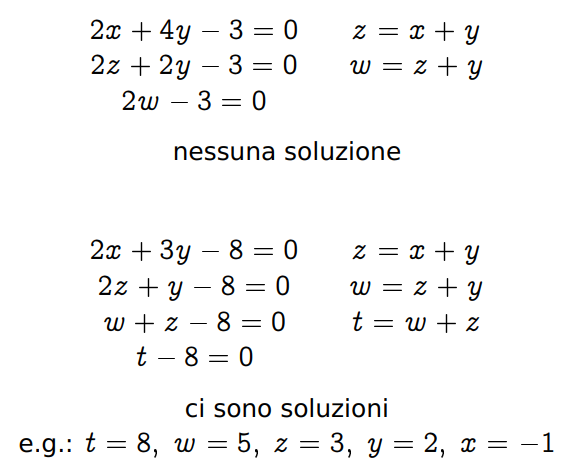
\includegraphics[width=8cm, keepaspectratio]{tesi_stile/img/dio1.png}
\end{figure}

\subsection{Teoria della Computabilità}
E se il 10th problema di Hilbert non avesse soluzione?\\
Dobbiamo rispondere alle domande:
\begin{enumerate}
    \item quali sono le funzioni per cui esiste un procedimento di calcolo effettivo?
    \item e quali quelle per cui un tale procedimento non esiste?
\end{enumerate}
Ma per rispondere alla domanda 2, è necessaria una \textbf{definizione formale di procedimento di calcolo effettivo}.\\\\
\textbf{Millennium prize problems (Millennium meeting Collège de France (Parigi), 24/5/2000)}\\
Il Clay Math. Institute (Boston) mette in palio 1.000.000\$ per chi risolve uno dei 7 problemi matematici più difficili.\\
Tra questi: \textbf{P vs. NP}

    \chapter{Cosa è un algoritmo}\label{ch:descrizione}
\section{Le regole di un algoritmo}
\begin{enumerate}
    \item Un algoritmo è di lunghezza finita.
    
    \item Esiste un agente di calcolo (la macchina calcolatrice, appunto) che sviluppa la computazione eseguendo le istruzioni dell’ algoritmo.
    
    \item L’agente di calcolo ha a disposizione una memoria, dove vengono immagazzinati i risultati intermedi del calcolo.
    
    \item Il calcolo avviene per passi discreti.
    
    \item Il calcolo non è probabilistico.
    
    \item Non deve esserci alcun limite finito alla lunghezza dei dati di ingresso.
    
    \item  Non deve esserci alcun limite alla quantità di memoria disponibile.
    
    \item Deve esserci un limite finito alla complessità delle istruzioni eseguibili dal dispositivo.
    
    \item Il numero di passi della computazione è finito ma non limitato.
    
    \item Sono ammesse computazioni senza fine.
\end{enumerate}

\section{Linguaggi Formali}
Ogni informazione può essere rappresentata da una sequenza finita di simboli su un opportuno alfabeto finito.\\\\
\textbf{Esempio.}\\La Divina Commedia, il genoma umano, i numeri interi e quelli razionali (per es. in base 10), grafi, polinomi, ecc... Possiamo quindi assumere che i processi di calcolo riguardino stringhe di simboli scelti in un insieme finito e non vuoto.

\subsection{Parole}
\textbf{Definizione}\\
Chiameremo alfabeto un insieme finito non vuoto A di simboli. I suoi elementi sono detti lettere.\\\\
\textbf{Esempi:}\\
$\{a, b\} , \{0, 1\} , \{a, b, c\} , \{0, 1, 2, 3, 4, 5, 6, 7, 8, 9, A, B, C, D, E,F\}$.\\\\
\textbf{Definizione}\\
Ogni sequenza finita di lettere di A si dice parola sull’alfabeto A. L’insieme delle parole sull’alfabeto A sarà denotato con A*.\\\\
\textbf{Esempi}\\
a, abb, ababbabb sono parole sull’alfabeto \{a, b\}.\\
01001010, 0110, 0000 sono parole sull’alfabeto \{0, 1\}.\\\\
Possiamo anche considerare la sequenza priva di lettere, che si denota con $\wedge$ (oppure $\epsilon$) e si dice parola vuota.

\newpage
\subsection{Lunghezza}
Una parola sull’alfabeto A è una sequenza u = a1a2...ak con k $>=$ 0, a1, a2, . . . , ak $\in$ A.\\\\
\textbf{Definizione}\\
\vspace{0.3cm}
L’intero k si dice lunghezza della parola u e si denota con l(u).\\\\
\textbf{Esempi}\\
l(a) = 1, l(aab) = 3, l(ababbabb) = 8, l($\wedge$) = 0.
\subsection{Concatenzione, fattori}
\textbf{Definizione}\\
Si considerino le parole u = a1a2...ak e v = b1b2...bh con k, h $>= 0$ \\
a1, a2, . . . , ak , b1, b2, ... ,bh $\in$ A.\\
La concatenazione di u e v è \textbf{la parola uv}:\\
\begin{center}
uv = a1a2...ak b1b2 ... bh.    
\end{center}
\textbf{Esempi}\\
La concatenazione delle parole abb e aaab è la parola abbaaab.\\
La concatenazione delle parole aaab e abb è la parola aaababb.\\
La concatenazione delle parole baa e $\wedge$ è la parola baa.\\\\ 
\textbf{Definizione}\\
Diremo che una parola v è un \textbf{fattore} di una parola w se risulta w = xvy.\\
Per opportune parole x , y. Nel caso in cui x = $\epsilon$ (risp., y = $\wedge$) il fattore v si dice 
prefisso (\textbf{risp}., \textbf{suffisso}) di w.\\ 
Diremo che v è un fattore proprio se v $\neq$ w.\\\\
\textbf{Esempio}\\
I fattori di abb sono $\wedge$, a, b, ab, bb e abb. Dove i prefissi sono $\wedge$, a, ab e abb ed i suffissi sono  $\wedge$, b, bb e abb.
\subsection{Linguaggio Formale}
\textbf{Definizione}\\
Ogni sottoinsieme di A* si dice linguaggio formale o linguaggio o problema sull’alfabeto A.\\\\
\textbf{Esempio}\\
Sono linguaggi formali sull’alfabeto A = \{a, b\}:\\
L0 = \{a, b\} , L1 = \{a, ab, abb\} , L2 = \{abna $|$ n $>=$ 0\} , L3 = $\emptyset$ , L4 = A*,\\L5 = \{a$^p$ $|$ p primo\}\\
Le espansioni binarie dei numeri primi costituiscono un linguaggio sull’alfabeto \{0,1\}.\\
L’insieme dei polinomi Diofantei nelle variabili x , $x'$, $x''$, $x'''$, . . . che ammettono una radice intera possono essere rappresentati come un linguaggio sull’alfabeto
\begin{center}
\{0, 1, 2, 3, 4, 5, 6, 7, 8, 9, $+$, $-$ ,$^\wedge$, x ,$"$\}
\end{center}

\subsection{Ordinamento}
\textbf{Definizione}\\
Sia A un alfabeto totalmente ordinato. L’ordine radicale (o militare) su A* è definito come segue:\\ 
siano u, v $\in$ A*.\\
Si ha u $<$ v se è soddisfatta una delle due condizioni seguenti:
\begin{itemize}
    \item l(u) $<$ l(v)
    
    \item l(u) = l(v) e u precede v nell’ordine lessicografico 
    
    (cioè u = ras, v = rbt con r,s,t $\in$ A* a, b $\in$ A e a $<$ b nell’ordinamento dell’alfabeto A)
\end{itemize}
\textbf{Esempio}\\
I numeri naturali sono rappresentati in base 10 da parole sull’alfabeto:
\begin{center}
    \{0, 1, 2, 3, 4, 5, 6, 7, 8, 9\}, prive di 0 iniziali.
\end{center}
L’ordinamento usuale dei numeri naturali coincide con ordine radicale delle corrispondenti espansioni decimali.

    \chapter{La Macchina di Turing} \label{ch:capitolo3}
\begin{figure}[htp]
    \centering
     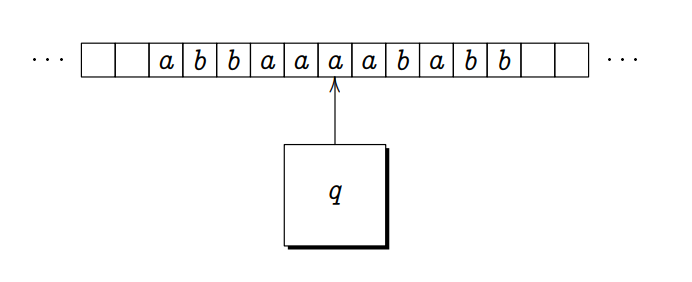
\includegraphics[scale=0.7]{tesi_stile/img/turing.png}
\end{figure}
E' composta da: 
\begin{itemize}
    \item un unità di controllo a stati finiti che
    \begin{itemize}
    
        \item può spostare il nastro a destra o a sinistra (una cella alla volta)
        
        \item contiene il programma secondo cui verrà eseguito il calcolo
        
        \item registra lo stato della macchina
        
        \item L’insieme di possibili stati della macchina è un insieme finito\\Q = \{q0, q1 ,. . . qn\}
    \end{itemize}
    \newpage
    \item un nastro di lunghezza infinita che
    
    \begin{itemize}
        \item è suddiviso in celle
        
        \item ogni cella può contenere un solo simbolo di un fissato alfabeto A, oppure essere bianca.
        
        \item  solo un numero finito di celle contiene una lettera di A.
    \end{itemize}
    
    \item Testina di lettura e scrittura
    
    \begin{itemize}
        \item che permette all’unità di controllo di leggere e scrivere un simbolo per volta dal nastro
    \end{itemize}
    
\end{itemize}
\subsection{Funzionamento}
All'avvio di ogni computazione, la macchina si trova in uno stato iniziale prefissato.\\ A ogni passo l’unità di controllo in funzione dello stato in cui si trova e del simbolo contenuto nella cella che la testina indica:
\begin{itemize}
    \item Rivede il suo stato.
    
    \item Scrive un simbolo nella cella indicata dalla testina, sostituendo il simbolo esistente (eventualmente bianco);
    
    \item Sposta la testina di una posizione a sinistra o a destra.
\end{itemize}
Il nuovo stato assunto dall'unità di controllo, il simbolo da scrivere sulla cella indicata dalla testina e lo spostamento della testina a sinistra o a destra sono determinati dal programma della macchina.
\newpage
\subsection{Programma}
Il programma di una macchina di Turing si può rappresentare come una lista di 5-ple (istruzioni):\\
$$(q,a,q',a',x)$$
\begin{itemize}
    \item q è lo stato dell'unità di controllo
    \item a l simbolo nella cella indicata dalla testina
    \item $q'$ l nuovo stato che la macchina deve assumere
    \item $a'$ la lettera da scrivere nella cella esaminata
    \item x è la testina. 
    
    Se $x = -1$ spostamento della testina a sx, $x = +1$ spostamento della testina a dx
\end{itemize} 
Per ogni coppia (q, a) ci deve essere al più una 5-pla (q, a, $q'$, $a'$, x ) nel programma della macchina \textbf{(determinismo)}
\subsection{Definizione Formale}
\textbf{Definizione}\\
Una macchina di Turing M è una quadrupla:
\begin{center}
    $$M=<Q,A,\delta,q_0>$$
\end{center}
\begin{itemize}
    \item $Q$ è un insieme finito di stati
    \item $A$ è un alfabeto a cui si aggiunge il simbolo \textit{bianco} \#
    \item $\delta$ è una funzione \textbf{parziale} da $Q \times (A \cup \{\# \})$ a \\
    $Q \times (A \cup \{\# \}) \times \{-1,+1\}$
    \item $q_0 \in Q$ è lo stato iniziale
\end{itemize}
Le 5-ple (q, a, $q'$, $a'$, x ) tali che $\delta$(q,a) = ($q'$, $a'$, x) sono dette \textbf{istruzioni} di M.
\subsection{Configurazione istantanea}
Lo stato di una Macchina di Turing a un dato istante può essere descritta da una 4-pla:
\begin{center}
   $$C_i = (\xi,q,a,\eta)$$ 
\end{center}
\begin{itemize}
    \item $\xi \ (xi)$ è il contenuto del nastro a sinistra della cella indicata dalla testina, privato della sequenza infinita di celle bianche che precedono l’ultimo simbolo non bianco. \emoji{orangutan}: $\xi$ contiene tutte le lettere a sinistra della testina fino alle infinite celle bianche (il nastro \`{e} infinito sia a destra che a sinistra)
    
    \item q è lo stato della Macchina di Turing nell’istante considerato
    
    \item a è la lettera nella cella indicata dalla testina
    
    \item $\eta \ (eta)$ è il contenuto del nastro a destra della cella indicata dalla testina, privato della sequenza infinita di celle bianche che seguono l’ultimo simbolo non bianco. \emoji{orangutan}: \`{e} come $\xi$ ma a destra
\end{itemize}
\textbf{Esempio}
\vspace{0.2cm}
\begin{figure}[htp]
    \centering
     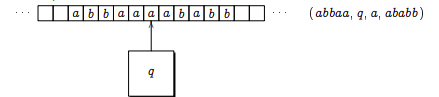
\includegraphics[scale=0.7]{tesi_stile/img/ese-turing.png}
\end{figure}
\newpage
\subsection{Configurazione consecutiva}
Una configurazione istantanea di una Macchina di Turing $$M=<Q,A,\delta,q_0>$$ è un elemento dell’insieme (A U \{\#\})* × Q × (A U \{\#\}) × (A U \{\#\})*.\\
Nell’insieme delle configurazioni istantanee di M introduciamo la relazione binaria  $\vdash_M$  che associa alla configurazione C quella che la segue nella computazione di M. Qualora tale configurazione non esistesse, scriveremo $\vdash/_M$.\\\\
\textbf{Esempio}\\
Se M ha l’istruzione (q, a, $q$, b, $-$1), allora:
\begin{center}
    (abbaa, q, a, ababb) $\vdash_M$ (abba, $q'$, a, bababb)
\end{center}
\subsection{Computazione}
\begin{itemize}
    \item Al passo iniziale 
    
    \begin{itemize}
    \item M esamina una parola w scritta sul nastro di input.
    
    \item La testina indica la prima lettera di w.
    
    \item Lo stato è lo stato iniziale q0.
    
    \item la configurazione istantanea iniziale è ($\wedge$, q0, a, $w'$), ove w = a$w'$ con a lettera
    \end{itemize}
\end{itemize}
\begin{itemize}
    \item Se all’istante i, M si trova nella configurazione C$_i$ e C$_i$  $\vdash_M$ C$_i$+1, allora all’istante i+1 M sarà nella configurazione C$_i$+1.
    
    \item Se invece C$_i$ $\vdash/_M$, allora la macchina si arresta.
    
    \item Se M si arresta dopo un numero finito di passi diremo che M converge sull’input w e scriveremo M $\downarrow$ w, in caso contrario diremo che M diverge sull’input w e scriveremo M $\uparrow$ w.
\end{itemize}
\newpage
\textbf{Esempio: bitwise not}
\begin{figure}[htp]
    \centering
     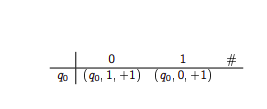
\includegraphics[scale=0.9]{tesi_stile/img/bit.png}
\end{figure}

\textbf{Esempio: palindrome}
\begin{figure}[htp]
    \centering
     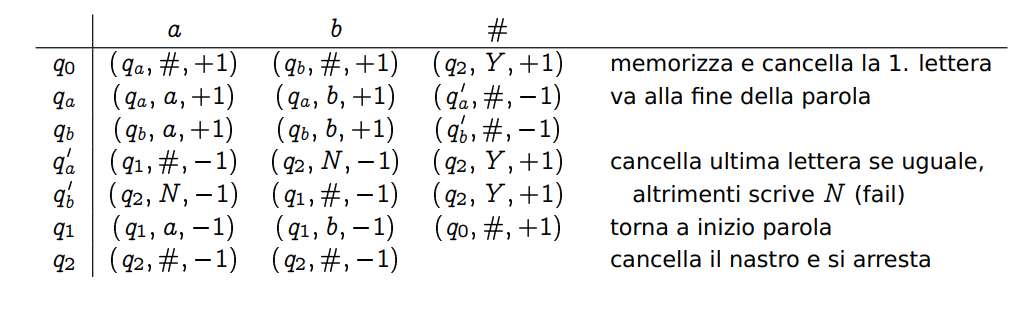
\includegraphics[scale=0.6]{tesi_stile/img/pal.png}
\end{figure}
\newpage
\subsection{Algoritmi e macchina di Turing}
\begin{figure}[htp]
    \centering
     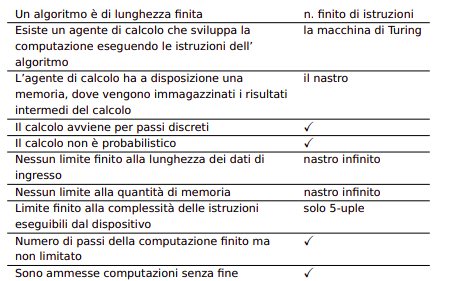
\includegraphics[scale=1]{tesi_stile/img/algo-turing.png}
\end{figure}
\subsection{L'impiegato diligente}
La macchina di turing è un Meccanismo che simuli le potenzialità computazionali dell’uomo comune quindi: 
\begin{itemize}
    \item Esegue ordinatamente le sue istruzioni, purché non siano tra loro in concorrenza.
    
    \item In assenza di istruzioni si arresta.
\end{itemize}
\newpage
\subsection{Macchina di turing e linguaggi}
Come detto in precendeza:
\begin{itemize}
    \item La configurazione istantanea iniziale è C0 = ($\wedge$, q0, a, $w'$), ove w = a$w'$
    con a lettera.
    
    \item Se C$_0$ $\vdash_M$ C$_1$ $\vdash_M$ ... $\vdash_M$ $C_n$ $\vdash/_M$ M allora M \textbf{converge} sull’input w.
    
    \item Se C$_0$ $\vdash_M$ C$_1$ $\vdash_M$ ... $\vdash_M$ $C_n$ $\vdash_M$ M allora M \textbf{diverge} sull’input w.
\end{itemize}
\textbf{Definizioni}\\
Sia L un linguaggio sull’alfabeto A.
\begin{enumerate}
    \item Una macchina di Turing M accetta il linguaggio L se M \textbf{converge su tutti gli input} w $\in$ L e \textbf{diverge} su tutti gli input w $\not \in$ L.
    
    \item Una macchina di Turing M decide il linguaggio L se M \textbf{converge su tutti gli input} w $\in$ A* con output SI se w $\in$ L e NO se w $\not \in$ L.
\end{enumerate}
\subsection{Problemi decidibili}
Le nozioni di linguaggio accettato e deciso sono profondamente diverse.
\begin{itemize}
    \item Entrambe definiscono correttamente un linguaggio.
    
    \item Solo la nozione di linguaggio deciso ci fornisce una procedura effettiva che, in un numero finito di passi, ci permette di dire se una parola appartiene o meno al linguaggio.
\end{itemize}
\textbf{Definizione}\\
Un linguaggio L si dice decidibile secondo Turing se esiste una macchina di Turing M che decide L, indecidibile (secondo Turing) altrimenti.\\
Un linguaggio L si dice semidecidibile secondo Turing se esiste una macchina di Turing M che accetta L.\\\\
\textbf{Proposizione}\\
Un linguaggio decidibile è anche semidecidibile\\\\
\textbf{Dimostrazione}\\
Trasformare la macchina che decide L in una che accetta L, aggiungendo un loop infinito se la macchina originale si arresta sul NO.\\\\
\textbf{Esempio}
\begin{figure}[htp]
    \centering
     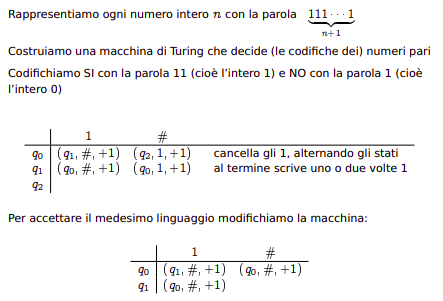
\includegraphics[scale=0.9]{tesi_stile/img/esempio.png}
\end{figure}
\subsection{Aritmetizzazione della macchina di turing}
\textbf{Obbietivo}\\
\begin{itemize}
    \item Associare un numero a ogni input e output di una macchina di Turing.
    
    \item Associare un numero (indice) a ogni macchina di Turing.
    
    \item In maniera effettiva:
    
    \begin{itemize}
        \item Data una macchina di Turing, ne posso calcolare l’indice.
        
        \item Dato un indice, posso calcolare le istruzioni della macchina corrispondente.
    \end{itemize}
\end{itemize}
\textbf{Una prima strategia}
\begin{itemize}
    \item Ordinare le parole nell’ordine militare.
    
    \item Associare a ogni parola la sua posizione nell’elenco ordinato.
\end{itemize}

Oppure

\begin{itemize}
    \item Interpretare ogni lettera come una cifra $\neq$ 0 di un sistema numerico.
    
    \item Associare a ogni parola il numero corrispondente.
\end{itemize}

\subsection{Numerazione di i Gödel}
Metodo per numerare gli alberi (con foglie etichettate).
\begin{figure}[htp]
    \centering
     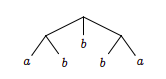
\includegraphics[scale=1]{tesi_stile/img/goedel.png}
\end{figure}
\begin{itemize}
    \item A ogni etichetta x associo un numero dispari G$_0$(x) $>=$ 3
    
    \item A un albero T di altezza 1, con foglie etichettate x$_1$, x$_2$, ... , x$_k$ associo il numero $$G_1(T) = 2^{G_0(x_1)} \cdot 3^{G_0(x_2)} \cdot 5^{G_0(x_3)} \cdot ... \cdot P_n^{G_0(x_k)}$$ dove 2, 3, ..., p$_k$ è la sequenza dei primi k numeri primi
    
    \item In generale, se la radice dell’albero T ha, da sinistra a destra, i figli v$_1$, . . . , v$_t$, radici di sottoalberi alberi con numeri di Gödel n$_1$, . . . , n$_t$, allora il numero di Gödel di T è 2$^{n1}$ 3$^{n2}$...p$_t^{ni}$
\end{itemize}
\newpage
\textbf{Esempio}\\
Posso anche fare il percorso inverso:
\begin{itemize}
    \item Un numero dispari rappresenta una foglia.
    
    \item Un numero pari va decomposto come prodotto di potenze di primi.
    
    \item Gli esponenti sono i numeri di Gödel dei sottoalberi
\end{itemize}
Posso quindi distinguere gli interi che non sono numeri di Gödel.\\\\
\begin{figure}[htp]
    \centering
     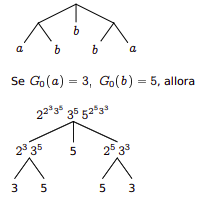
\includegraphics[scale=1]{tesi_stile/img/inverso.png}
\end{figure}\\
\textbf{Il Teorema Fondamentale dell’Aritmetica assicura che la decodifica è unica.}
\newpage
\subsection{Numerazione della macchina di turing}
Una macchina di Turing è rappresentata da una lista di 5-ple e, in definitiva, da un albero.\\\\
\textbf{Esempio}\\
La macchina che accetta i numeri pari ha le 5-ple (in ordine lessicografico).\\
\begin{center}
    (q$_0$, \#, q$_0$, \#, $+1$),(q$_0$, 1, q$_1$, \#, $+1$),(q$_1$, 1, q$_0$, \#, $+1$)
\end{center}
Possiamo identificarlo come albero:
\begin{figure}[htp]
    \centering
     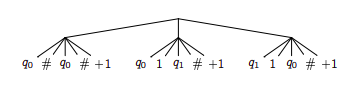
\includegraphics[scale=1]{tesi_stile/img/albero.png}
\end{figure}\\
Per numerare le macchine di Turing su un alfabeto A,\\ 
associamo: un intero dispari $>$ 1 a ognuno dei simboli necessari.\\
\begin{figure}[htp]
    \centering
     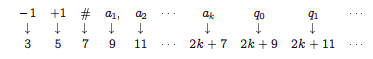
\includegraphics[scale=0.8]{tesi_stile/img/numeri.png}
\end{figure}
\newpage
Per ogni macchina di Turing M:
\begin{itemize}
    \item Ordiniamo le 5-ple in ordine lessicografico.
    
    \item Calcoliamo il numero di Gödel dell’albero corrispondente.\\
    \begin{figure}[htp]
        \centering
        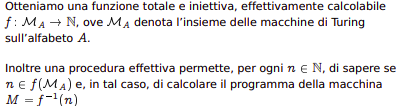
\includegraphics[scale=0.9]{tesi_stile/img/sotto.png}
     
    \end{figure}
\end{itemize}
\begin{figure}[htp]
    \centering
    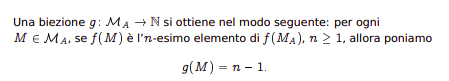
\includegraphics[scale=0.9]{tesi_stile/img/biiezione.png}
\end{figure}
\textbf{Osservazione}\\
Una procedura effettiva per calcolare x = g(M) è la seguente:
\begin{figure}[htp]
    \centering
    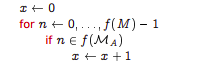
\includegraphics[scale=0.8]{tesi_stile/img/algoritmo.png}
\end{figure}\\
\textbf{Teorema}\\
C’è una corrispondenza biunivoca effettiva tra le macchine di Turing su un alfabeto A e i numeri naturali.
\newpage
\subsection{Coppie di interi}
\textbf{Teorema di Cantor:} Esiste una biiezione effettiva tra $N^2$ ed $N$ data da:\\
$$(n,m)=\frac{(n+m)(n+m+1)}{2}+n$$
Basta osservare che ogni naturale compare infinite volte come ascissa di una coppia $(n,m) \in N^2$ al variare di $m$, intuitivamente quindi ci sono tante coppie ordinate di naturali quanti naturali.
\begin{figure}[htp]
    \centering
    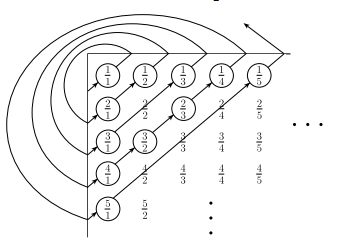
\includegraphics[scale=0.9]{tesi_stile/img/cantor.png}
\end{figure}\\
\textbf{Corollario}\\
C’è una corrispondenza biunivoca effettiva tra le macchine di Turing su qualsiasi alfabeto e i numeri naturali.
Per il teorema precedente possiamo enumerare le macchine di Turing
\begin{center}
    M$_0$,M$_1$,...,    M$_n$
\end{center}
Pertanto, è possibile enumerare tutte le funzioni calcolabili
\begin{center}
    $\phi_0$,$\phi_1$,...,$\phi_n$
\end{center}
Nel secondo caso, però, la corrispondenza non è biunivoca, perchè la medesima funzione può essere calcolata da più macchine di Turing.
\subsection{Descrizione delle macchine di turing}
\textbf{Descrizione formale}\\
Lista delle quintuple\\\\
\textbf{Descrizione implementativa}\\
Descrive in linguaggio corrente, il modo in cui la macchina di Turing muove la testina e registra i dati sul nastro\\\\
\textbf{Descrizione di alto livello}\\
Descrive un algoritmo, ignorando i dettagli implementativi.\\\\
\textbf{Esempio}: Palindrome\\\\
Descrizione implementativa su input w
\begin{enumerate}
    \item cancella la prima lettera
    
    \item se non ci sono altre lettere accetta
    
    \item sposta la testina alla fine della parola
    
    \item se l’ultima lettera è diversa dalla prima rifiuta
    
    \item cancella l’ultima lettera
    
    \item se non ci sono altre lettere accetta
    
    \item sposta la testina all’inizio della parola
    
    \item ricomincia dal passo 1
\end{enumerate}
Descrizione di alto livello su input w
\begin{enumerate}
    \item se l(w) $<=$ 1, accetta
    
    \item se la prima e l’ultima lettera di w sono distinte, rifiuta
    
    \item cancella la prima e l’ultima lettera di w
    
    \item ricomincia al passo 1
\end{enumerate}
\subsection{Tesi di Church-Turing}
Una funzione è calcolabile se e solo se esiste una macchina di Turing che la calcola.
\begin{figure}[htp]
    \centering
    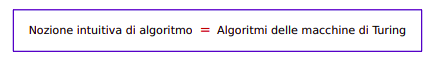
\includegraphics[scale=0.8]{tesi_stile/img/tesi.png}
\end{figure}
\textbf{Argomenti}
\begin{itemize}
    \item L’inclusione $\supseteq$ è evidente
    
    \item Assenza di controesempi
    
    \item Tecniche molto generali
    
    \item Numerosi modelli equivalenti
    
    \item Numerose generalizzazioni rivelatesi equivalenti
    
    \item La metafora dell’impiegato diligente
\end{itemize}
\textbf{Convenzione}\\
D’ora in poi considereremo solo insiemi di numeri naturali e funzioni di $N$ in $N$ (ipotesi non restrittiva). Le macchine di Turing si enumerano
\begin{center}
    M$_0$,M$_1$,...,M$_n$
\end{center}
e le funzioni da esse calcolate saranno denotate, rispettivamente
\begin{center}
    $\phi_0$,$\phi_1$,...,$\phi_n$
\end{center}
\textbf{Osservazioni}
\begin{itemize}
    \item Ogni macchina di Turing calcola una funzione (parziale) di $N$ in $N$
    
    \item Ogni macchina di Turing calcola una funzione (parziale) di $N^2$ in N
    
    \item Esiste una procedura effettiva che, data una macchina di Turing M, calcola l’indice x tale che M = M$_x$
    
    \item Esiste una procedura effettiva che, dato un numero naturale x , calcola il programma della macchina di Turing M$_x$
\end{itemize}
\subsection{Funzioni e problemi}
La funzione caratteristica di un insieme L $\subseteq$ $N$ è la funzione f$_L$ definita da:
\begin{figure}[htp]
    \centering
    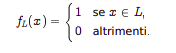
\includegraphics[scale=0.9]{tesi_stile/img/funzione.png}
\end{figure}
\textbf{Lemma}\\
Un insieme L $\subseteq$ $N$ è decidibile se e solo se la sua funzione caratteristica è computabile.\\\\
\textbf{Corollario:} Esistono insiemi indecidibili\\\\
\textbf{Dimostrazione}\\
Per il Teorema di Cantor, non ci sono ‘abbastanza’ macchine di Turing.\\\\
\textbf{Esempio}
\begin{figure}[htp]
    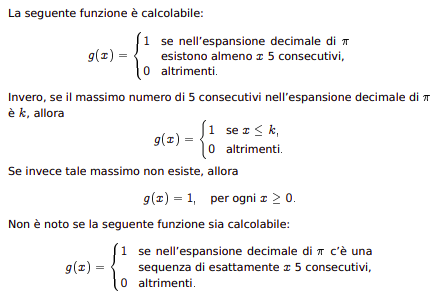
\includegraphics[scale=1]{tesi_stile/img/es-cantor.png}
\end{figure}
    \chapter{Problemi insolubili} \label{ch:capitolo4}
\subsection{La macchina di turing Universale}
\textbf{Teorema}\\
La funzione g : $N^2 \mapsto N$ definita ponendo, per ogni x , y $\in$ $N$
\begin{center}
    g(x,y) = $\phi_x$(y)
\end{center}
è calcolabile secondo turing.\\\\
\textbf{Dimostrazione}
Su un input (x,y) $\in$ $N^2$
\begin{enumerate}
    \item Decodifica le istruzioni di M$_x$
    
    \item Simula M$_x$ sull’input y
    
    \item Se M$_x$ si arresta, restituisci l’output della computazione
\end{enumerate}
\textbf{Definizione}\\
La macchina di Turing $\mu$ che calcola la funzione g si dice Macchina di Turing universale.\\
La macchina di Turing universale ha la capacità di eseguire qualunque algoritmo.\\
Calcolatore all purpose (modello di Von Neumann).
\newpage
\subsection{La diagonalizzazione}
\textbf{Teorema}
L'insieme $R$ non è numerabile.\\\\
\textbf{Dimostrazione}\\
Per assurdo. Se $R$ fosse numerabile, avremmo una tabella infinita con tutti i numeri reali:\\
\begin{figure}[htp]
    \centering
    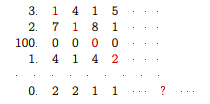
\includegraphics[scale=0.8]{tesi_stile/img/diagonalizzazione.png}
\end{figure}\\
Costruiamo un numero reale x = 0,c$_1$,c$_2$,c$_3$ ... in cui la i-esima cifra decimale è diversa dalla i-esima cifra rossa (e anche da 0 e 9).\\
Per esempio: 0.2211 ...\\
Dove può comparire nella nostra tabella?
\newpage
\subsection{Il problema dell'arresto}
Data una macchina di Turing M e un input y, decidere se M si arresta sull’input y.\\
\begin{center}
    H = \{(x,y) $\in$ $N^2$ $|$ M$_x$ $\downarrow$ y\}
\end{center}
\begin{figure}[htp]
    \centering
    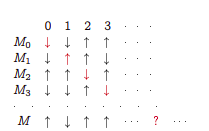
\includegraphics[scale=0.8]{tesi_stile/img/arresto.png}
\end{figure}
Se sapessi risolvere il problema dell’arresto, potrei costruire una macchina di Turing M che su ciascun input x si arresta se e solo se l’elemento x-esimo della diagonale è $\uparrow$.\\
Come prima, tale macchina non può comparire nella nostra tabella!\\
\textbf{Teorema}\\
Il problema dell’arresto non è decidibile.\\\\
\textbf{Dimostrazione}\\
Per assurdo supponiamo che H sia decidibile.\\
Allora anche il problema:
\begin{center}
    K = \{ x $\in$ N $|$ (x , x ) $\in$ H\}
\end{center}
è decidibile.\\
Invero, sia M una macchina di Turing che decide H. Il problema H è deciso dalla macchina M$'$ che esegue il seguente programma:\\
Su input x $\in$ $N$
\begin{center}
    \begin{enumerate}
        \item simula M su (x , x )
        
        \item restituisci l’output della computazione
    \end{enumerate}
\end{center}
\subsection{Il problema dell'arresto2}
Anche il complemento di K è decidibile e, di conseguenza semidecidibile. Più precisamente, K è accettato dalla macchina M$"$ che esegue il seguente programma.\\
Su input x $\in$ $N$
\begin{center}
    \begin{enumerate}
        \item Simula M su (x , x )
        
        \item Se l’output è NO, accetta; se l’output è SI, eseguire un loop infinito
    \end{enumerate}
\end{center}
Sia z l’indice della macchina M$"$. Allora\\
\begin{figure}[htp]
    \centering
    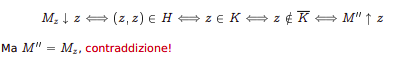
\includegraphics[scale=1]{tesi_stile/img/contraddizione.png}
\end{figure}
\subsection{Riduzioni}
Siano S e T due problemi. Una funzione totale e calcolabile $f$:$N$$\rightarrow$$N$ si dice riduzione del problema S al problema T se, per ogni x $\in$ N si ha:
\begin{center}
    x $\in$ S se e soltanto se $f(x)$ $\in$ T
\end{center}
\textbf{Proposizione}\\
Siano S e T due problemi. Se esite una riduzione di S a T e T è decidibile, allora S è decidibile.\\\\
\textbf{Dimostrazione}\\
Siano M e M$'$ rispettivamente la macchina di Turing che calcola f e quella che decide T. Allora S è deciso dalla macchina che esegue il seguente algoritmo.\\
Su input x
\begin{enumerate}
    \item simula M su x
    
    \item simula M$'$ sull’output di M
    
    \item restituisci l’output di M$'$
\end{enumerate}
\subsection{Riduzioni-2}
\textbf{Corollario}\\
Siano S e T due problemi. Se esite una riduzione di S a T e S è indecidibile, allora anche T è indecidibile.\\\\
\textbf{Proposizione}\\
Siano S e T due problemi. Se esite una riduzione di S a T e T è semidecidibile, allora S è semidecidibile.\\\\
\textbf{Esempio}\\
La funzione x $\in$ $N \mapsto (x,x)$ $\in$ $N^2$ è una riduzione del problema K al problema dell’arresto H.\\\\
\textbf{Osservazione}\\
Il problema dell’arresto è semi-decidibile.\\
Invero, è accettato dalla macchina di Turing universale.\\
\begin{center}
    Il problema\{(x,y, z) $\in$ $N^3$ $|$ M$_x$ $\downarrow$ y in al più z passi\}  \textbf{è decidibile}
\end{center}
\textbf{Teoria della programmazione}\\
Non è possibile costruire un sistema di debugging in grado di stabilire se un
programma termini o meno
\newpage
\subsection{Equivalenza di macchine di Turing}
\textbf{Problema dell’equivalenza di macchine di Turing}\\
Date due macchine di Turing, decidere se calcolano la medesima funzione:
\begin{center}
    E = \{(x , y) $|$ $\phi_x$ = $\phi_y$\}.
\end{center}
\textbf{Osservazione}\\
Due funzioni sono uguali se
\begin{itemize}
    \item hanno lo stesso dominio,
    
    \item hanno lo stesso valore su ogni elemento del dominio.
\end{itemize}
La dimostrazione richiede vari passi che utilizzano diagonalizzazione e riduzione
\newpage
\subsection{Funzioni Totali}
\textbf{Proposizione}\\
Il problema T = \{x $\in$ N $|$ $\phi_x$ è totale\} è indecidibile.\\\\
\textbf{Dimostrazione}\\
Per assurdo, sia T decidibile.\\
Allora c’è una funzione calcolabile totale f tale che T = f($N$).\\
Invero f è calcolata dal seguente algoritmo\\
\begin{figure}[htp]
    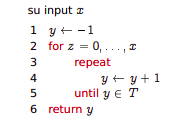
\includegraphics[scale=1]{tesi_stile/img/algo.png}
\end{figure}\\
La funzione g : $N$ $\mapsto$ $N$ definita da
\begin{center}
    g(x) = $\phi_f(x)$ (x)$+$1
\end{center}
è calcolabile totale. Pertanto, g = $\phi_f(z)$ per un opportuno z $\in$ $N$.\\
\begin{figure}[htp]
    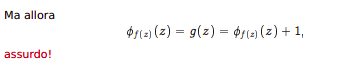
\includegraphics[scale=1]{tesi_stile/img/assurdo.png}
\end{figure}
\newpage
\subsection{Funzione Nulla}
La funzione nulla è la funzione calcolabile totale Z : x $\in$ N $\mapsto$ 0.\\\\
\textbf{Proposizione}\\
Per ogni x $\in$ N, consideriamo la funzione g$_x$ definita da:\\
\begin{figure}[htp]
    \centering
    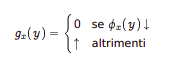
\includegraphics[scale=1]{tesi_stile/img/nulla.png}
\end{figure}\\
Si verifica facilmente che g$_x$ è calcolabile e anche il suo indice è calcolabile.\\
Invero esso è calcolato dal seguente algoritmo:\\
Su input x
\begin{center}
    \begin{enumerate}
        \item calcola il programma di M$_x$
        
        \item aggiungi al programma le istruzioni seguenti:
        \begin{itemize}
            \item se la macchina originale si arresta, output zero
        \end{itemize}
        \item restituisci il codice della macchina modificata
    \end{enumerate}
\end{center}
Quindi g$_x$ = $\phi_h(x)$, con h calcolabile totale. Inoltre\\
\begin{figure}[htp]
    \centering
    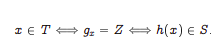
\includegraphics[scale=1]{tesi_stile/img/nulla2.png}
\end{figure}\\
Pertanto h è una riduzione di T a S.\\
Poiché T è indecidibile, lo sarà anche S.
\newpage
\subsection{Equivalenza di macchine di Turing}
\textbf{Proposizione}\\
Il problema E = \{(x , y) $\in$ $N^2$ $|$ $\phi_x$ = $\phi_y$\} è \textbf{indecidibile}\\\\
\textbf{Dimostrazione}\\
Sia z l’indice della funzione nulla.\\
La funzione f : x $\in$ N $\mapsto$ (x,z) $\in$ $N^2$ è una riduzione di S a E.\\
Poiché S è indecidibile, lo sarà anche E.\\\\
\textbf{Osservazione}\\
Non è possibile decidere se due generici programmi calcolano la stessa funzione: la correttezza semantica di un programma è indecidibile.







    \chapter{Problemi semi-decidibili} \label{ch:capitolo5}
\subsection{Insiemi semi-decidibili}
\textbf{Definizione}\\
Un problema L $\subseteq$ N è decidibile se esiste una macchina di Turing che computa la sua funzione caratteristica\\
\begin{figure}[htp]
    \centering
    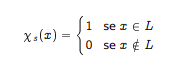
\includegraphics[scale=0.8]{tesi_stile/img/sem1.png}
\end{figure}
Il problema L è \textbf{semidecidibile} se esiste una macchina di Turing M che accetta L, ovvero, per ogni x $\in$ N,
\begin{center}
    M $\downarrow$ x se e solo se x $\in$ L
\end{center}
\textbf{Teorema}\\
Sia L  $\subseteq$ N. Allora le proposizioni seguenti sono equivalenti:
\begin{itemize}
    \item L è semidecidibile
    
    \item L è il dominio di una funzione calcolabile
    
    \item L è vuoto o c’è una funzione totale calcolabile $f : N \mapsto N$ tale che $L = f (N)$
\end{itemize}
\newpage
\subsection{Enumerabilità effettiva}
\textbf{Osservazione}\\
Se $L\neq\emptyset$, la condizione 3 esprime il fatto che esiste una enumerazione effettiva degli elementi di L:
\begin{center}
    f(0),f(1),f(2), . . . , f (n), . . .
\end{center}
\textbf{Dimostrazione}
\begin{enumerate}
    \item L è semidecidibile
    
    \item L è il dominio di una funzione calcolabile
    
    \item L è vuoto o c’è una funzione totale calcolabile $f : N \mapsto N$ tale che $L = f (N)$
\end{enumerate}
L’equivalenza tra 1 e 2 è immediata.\\
Mostriamo che 1 implica 3. Se $L\neq\emptyset$ è accettato dalla macchina di Turing M , allora la seguente procedura infinita produce tutti gli elementi di L (con ripetizioni).\\
\begin{figure}[htp]
    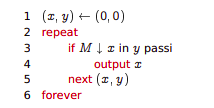
\includegraphics[scale=0.8]{tesi_stile/img/semi2.png}
\end{figure}
(next genera la coppia successiva in una enumerazione di $N x N$)\\
Poniamo $f(x)$ uguale all’($x+1$)-esimo output della procedura precedente.\\
Mostriamo che 3 implica 1. Se $L = f (N)$, allora L è accettato dalla macchina di Turing che esegue il seguente algoritmo.
\begin{figure}[htp]
    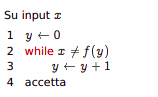
\includegraphics[scale=0.8]{tesi_stile/img/semi3.png}
\end{figure}
\subsection{Insiemi semidecidibili e decidibili}
\textbf{Teorema}\\
Un insieme L è decidibile se e solo se sia L che il suo complemento sono semidecidibili.\\\\
\textbf{Dimostrazione}\\
Se L è decidibile, lo è anche il complemento. Pertanto, sono semidecidibili entrambi.\\
Viceversa, se L e il suo complemento sono accettati dalle macchine di Turing $M$ e $M'$, rispettivamente, la seguente procedura decide L:\\
\begin{figure}[htp]
    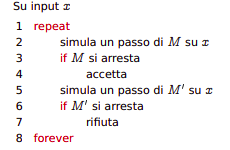
\includegraphics[scale=0.8]{tesi_stile/img/official.png}
\end{figure}\\
\textbf{Esempio}\\
Il problema:
\begin{center}
    K = \{$x \in N | M_x \downarrow x $\}
\end{center}
è semidecidibile ma non decidibile (invero è riducibile al problema dell’arresto, che è semidecidibile in quanto accettato dalla macchina di Turing universale).\\
Pertanto:\\
\begin{center}
    $\overline{k}$ = \{$x \in N | M_x \uparrow x $\}
\end{center}
non è semidecidibile.\\
\textbf{Osservazione}\\
Esistono macchine di Turing M per cui è indecidibile il problema.
\begin{center}
    \{$x \in N | M \downarrow x$\}.
\end{center}
In effetti, qualunque macchina di Turing che accetti un linguaggio semidecidibile ma non decidibile (come, ad es., K ) ha questa proprietà.
\subsection{Il 10 problema di Hilbert}
Data un’equazione Diofantea, determinare se ammette soluzioni intere.\\
Il problema seguente si riduce al decimo problema di Hilbert.\\\\
\textbf{Problema}\\
Data un’equazione Diofantea, determinare se ammette soluzioni in numeri naturali\\\\
\textbf{Dimostrazione}\\
L’equazione
\begin{center}
    $D(x,y,z) = 0$
\end{center}
ha una soluzione naturale se e soltanto se l’equazione.\\
\begin{center}
    $D(x^2_1 + x^2_2 + x^2_3 + x^2_4, y^2_1 + y^2_2 + y^2_3 + y^2_4, z^2_1 + z^2_2 + z^2_3 + z^2_4) = 0$
\end{center}
ha una soluzione intera (per il Teorema dei quattro quadrati di Lagrange).
\subsection{Insiemi diofanteei}
\textbf{Definizione}\\
Un insieme $L \subseteq N$ si dice Diofanteo se esiste un’equazione Diofantea $D(x_0, x_1, . . . , x_m) = 0$ tale che
\begin{center}
    $L = \{a \in N | D(a, x_1, . . . , x_m ) = 0$ ha soluzione\}
\end{center}
\textbf{Osservazione}\\
Una soluzione del 10. problema di Hilbert implicherebbe la decidibilità di tutti gli insiemi Diofantei.\\\\
\textbf{Esempi}\\
L’insieme dei quadrati perfetti è rappresentato da
\begin{center}
    $a - x^2 = 0$
\end{center}
L’insieme dei numeri composti è rappresentato da
\begin{center}
    $a - (x_1 + 2)(x_2 + 2) = 0$
\end{center}
L’insieme dei numeri che non sono potenze di 2 è rappresentato da
\begin{center}
    $a - (2x_1 +3)x_2 = 0$
\end{center}
\textbf{Proposizione}\\
Gli insiemi Diofantei sono semidecidibili. (perchè è semidecidibile il 10. problema di Hilbert)
\subsection{Insiemi Diofantei e insiemi semidecidibili}
\textbf{Osservazione}\\
L’equazione $D(a, x_1, . . . , x_m ) = 0$ ha soluzioni se e solo se ha soluzioni l’equazione:
\begin{center}
    $a = (x_0 + 1)(1 - (D(x_0, x_1, . . . , x_m))2) - 1$
\end{center}
Quindi, un insieme Diofanteo è l’insieme dei valori positivi assunti da un polinomio con variabili in N.\\\\
\textbf{Congettura di M. Davis}\\
\begin{figure}[htp]
    \centering
    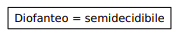
\includegraphics[scale=0.9]{tesi_stile/img/semi6.png}
\end{figure}\\
\textbf{Teorema (M. Davis, H. Putnam, J. Robinson)}\\
Per ogni insieme semidecidibile L esiste un’equazione Diofantea esponenziale E tale che
\begin{center}
    $L = \{a \in N | E ha una soluzione (a, x_1, . . . , x_n )\}$
\end{center}
Un’equazione Diofantea esponenziale è, ad esempio
\begin{center}
    $(x + 1)^{y+2} + x^3 = y^{(x+1)^x}+ y^4$
\end{center}
\subsection{Prova della congettura di Davis}
Come corollario del teorema di Davis, Putnam e Robinson, per provare la congettura di Davis ci si può ridurre al solo insieme:
\begin{center}
    ${(a, b, a^b) | a, b \in N}$
\end{center}
Il fatto che quest’ultimo insieme è Diofanteo è stato definitivamente dimostrato da Y. Matiyasevich (1970).\\\\
\textbf{Teorema (Davis, Putnam, Robinson, Matiyasevich)}\\
Ogni insieme semidecidibile è Diofanteo. Pertanto il 10. problema di Hilbert è indecidibile.\\\\
\textbf{Osservazione}\\
L’intera teoria della computabilità si può riscrivere in termini di equazioni Diofantee.\\\\
\textbf{Problema}\\
Data un’equazione Diofantea, determinare se ammette soluzioni razionali.





    \chapter{Auto-riferimento} \label{ch:capitolo6}
\section{Autoriferimento}
\subsection{Teorema di ricursione di Turing}
\textbf{Teorema}\\
Sia $f: N $ x $N \mapsto N$ una funzione calcolabile (parziale). Esiste effettivamente $z \in N$ tale che:
\begin{center}
    $\phi_z (y) = f(z,y).$
\end{center}
\textbf{Osservazione}
\begin{itemize}
    \item Il programma di una macchina di Turing può accedere al suo codice
    
    \item Si può calcolare una funzione che dipende anche dalla macchina che la calcola
\end{itemize}
\textbf{Esempio}\\
Cosa calcola la seguente macchina di Turing?.\\
Su input x
\begin{figure}[htp]
    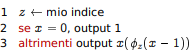
\includegraphics[scale=0.8]{tesi_stile/img/cap6f1.png}
\end{figure}
\subsection{Teorema s-m-n}
\textbf{Teorema}\\
Sia $f : N $ x $N \mapsto N$ una funzione (parziale) calcolabile. Allora esiste una funzione calcolabile totale $t:N \mapsto N$ tale che
\begin{center}
    $\phi_{t(x)} (y)=f(x,y)$ con $x,y \in N.$
\end{center}
\textbf{Osservazione}\\
Questo teorema ci dice che ogni funzione di due variabili f(x,y) si può calcolare nel modo seguente:
\begin{itemize}
    \item costruisco una macchina di Turing $M = M_t(x)$ che dipende solo da x
    
    \item eseguo M sull'input y
\end{itemize}
\newpage
\subsection{Dimostrazione del Teorema s-m-n}
\textbf{Dimostrazione}\\
Per ogni $x \in N,$ sia $g_x: N \mapsto N$ la funzione definita da $g_x(y) = f(x,y)$.\\\\
Una macchina di Turing per calcolare gx si ottiene concatenando
\begin{itemize}
    \item le istruzioni per stampare x sul nastro prima di y
    
    \item le istruzioni della macchina di Turing che calcola f .
\end{itemize}
Dato x, si può effettivamente costruire tale macchina e calcolarne l’indice.\\
Se t è la funzione che esegue questo calcolo, si avrà\\
\begin{center}
    $f(x,y)=g_x(y) = \phi_{t(x)}(y).$\\
\end{center}
\begin{figure}[htp]
    \centering
    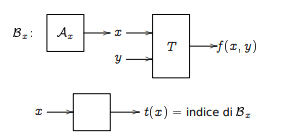
\includegraphics[scale=0.8]{tesi_stile/img/cap6foto2.png}
\end{figure}
\newpage
\subsection{Dimostrazione del Teorema di Ricursione}
Per ogni $x \in N$, sia $g_x : N \mapsto N$ la funzione definita da $g_x(y) = f(x,y)$.
\begin{figure}[htp]
    \centering
    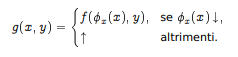
\includegraphics[scale=0.9]{tesi_stile/img/cap6f3.png}
\end{figure}
\\Una macchina di Turing per calcolare $g_x$ si ottiene concatenando.\\
Per il Teorema s-m-n, c’è una funzione totale t = $\phi_v$ tale che\\
\begin{center}
    $\phi_{t(z)}(y) = g(x,y)$ con $x,y \in N$
\end{center}
Posto $z = t(v) = \phi_v (v)$, si ha
\begin{center}
   $ \phi_z(y) = \phi_t{(v)}(y) = g(v,y)=f(\phi_v(v), y) = f (z,y)$
\end{center}
\newpage
\subsection{Costruzione}
\begin{figure}[htp]
    \centering
    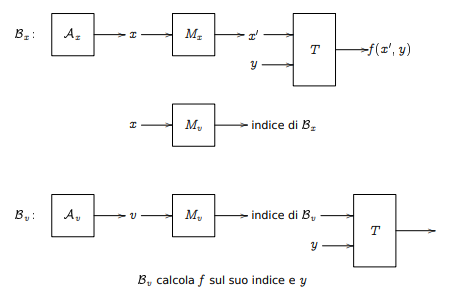
\includegraphics[scale=1]{tesi_stile/img/cap6f4.png}
\end{figure}
\newpage
\subsection{Esempio}
È indecidibile se una macchina di Turing accetta 1.\\
Se così non fosse, potremmo costruire una macchina di Turing con il seguente programma\\
Su input x.\\
\begin{figure}[htp]
    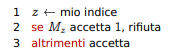
\includegraphics[scale=0.8]{tesi_stile/img/cap6f5.png}
\end{figure}\\
\begin{center}
    \textbf{Contraddizione!}
\end{center}
Nuova dimostrazione dell’indecidibilità del problema dell’arresto:\\
Se fosse decidibile, potremmo costruire una macchina di Turing con il seguente programma.\\
Su input x.\\
\begin{figure}[htp]
    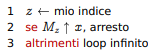
\includegraphics[scale=0.8]{tesi_stile/img/cap6f6.png}
\end{figure}\\
\begin{center}
    \textbf{Contraddizione!}
\end{center}
\newpage
\subsection{Teorema del punto fisso}
\textbf{Teorema}\\
 Sia $t : N \mapsto N$ una funzione calcolabile totale.\\
 Esiste effettivamente $z \in N$ tale che\\
 \begin{center}
     $\phi_z = \phi_t(z)$
 \end{center}
 \textbf{Dimostrazione}\\
La funzione $f : N$ x $N \mapsto N$ definita da $f(x,y) = \phi_{t(x)}(y)$ con $x,y \in N$, è
calcolabile. Per il Teorema di Recursione ci sarà $z \in N$ tale che\\
\begin{center}
    $\phi_z (y) = f (z,y) = \phi_t(z) (y),  y \in N.$
\end{center}
\textbf{Oppure}\\
Basta considerare la funzione calcolata dalla procedura.\\
Su input x\\
\begin{figure}[htp]
    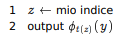
\includegraphics[scale=0.8]{tesi_stile/img/cap6f7.png}
\end{figure}
\newpage
\subsection{Teorema di Radice}
\textbf{Teorema}\\
Sia P una famiglia di funzioni calcolabili. L’insieme.\\
\begin{center}
    $R = \{x \in N | \phi_x \in P\}$
\end{center}
è indecidibile, purchè $R\neq \varnothing$, $N$.\\\\
\textbf{Dimostrazione}\\
Per assurdo, supponiamo che R sia decidibile e $R \neq \varnothing$, $N$. 
\begin{itemize}
    \item Possiamo trovare $i \in R$ e $j \notin R$.
    
    \item Definiamo la funzione $f : N $ x $N \mapsto N$ con
\end{itemize}
\begin{figure}[htp]
    \centering
    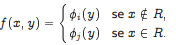
\includegraphics[scale=0.8]{tesi_stile/img/cap6f8.png}
\end{figure}
Per il Teorema di Recursione ci sarà $z \in N$ tale che $\phi_z (y) = f(z,y)$.\\
Ma allora se $z \notin R$, si ha $\phi_z = \phi_i \in R$, mentre se $z \in R$, si ha $\phi_z = \phi_j \notin R$.\\
\begin{center}
    \centering
    \textbf{Contraddizione!}.
\end{center}
\newpage
\subsection{Macchina di Turing minimali}
\textbf{Definizione}\\
Una macchina di Turing è minimale se non esistono macchine di Turing con un minor numero di stati che calcolano la stessa funzione.\\\\
\textbf{Osservazione}\\
Legata alle nozioni di complessità di Kolmogorov, entropia, compressibilità.\\\\
\textbf{Proposizione}\\
È indecidibile se una macchina di Turing è minimale.\\\\
\textbf{Dimostrazione}\\
Se così non fosse, avremmo una macchina di Turing che:\\
Su input x
\begin{figure}[htp]
    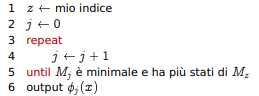
\includegraphics[scale=0.8]{tesi_stile/img/cap6f9.png}
\end{figure}
\\Ma allora Mz è equivalente a una macchina minimale con più stati: \textbf{assurdo}
    \chapter{Il problema di corrispondenza di post} \label{ch:capitolo7}
\subsection{PCP}
Un’istanza del problema di corrispondenza di Post (PCP)è una ($2$n)-pla di parole:
\begin{center}
    ($u_1, v_1; u_2, v_2;...;u_n,v_n$)
\end{center}
Su un alfabeto A, $n >= 1$.\\
Un match di tale istanza è una sequenza $i_1, i_2,...,i_k$ con$ k > 0$, tale che
\begin{center}
    $u_{i1},u_{i2} ... u_{ik} = v_{i1},v_{i2} ... v_{ik}$
\end{center}
Denotiamo con PCP l’insieme delle istanze che hanno un match.\\\\
\textbf{Osservazione}\\
In termini algebrici, PCP è l’insieme delle coppie di omomorfismi di semigruppi liberi $g, h : B^+ \mapsto A^+$ che coincidono almeno su una parola di $A^+$.
\newpage
\subsection{Problema corrispondenza di post}
\textbf{Esempio}\\
Consideriamo l’istanza (b,ca;a,ab;ca,a;abc,c) che possiamo rappresentare nella forma
\begin{figure}[htp]
    \centering
    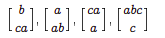
\includegraphics[scale=0.8]{tesi_stile/img/cap7f1.png}
\end{figure}\\
Un match si ottiene concatenando
\begin{figure}[htp]
    \centering
    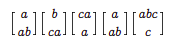
\includegraphics[scale=0.8]{tesi_stile/img/cap7f2.png}
\end{figure}\\
\textbf{Esempio}\\
L’istanza\\
\begin{figure}[htp]
    \centering
    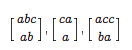
\includegraphics[scale=0.8]{tesi_stile/img/cap7f3.png}
\end{figure}\\
non ha match.\\\\
\textbf{Teorema}\\
PCP è indecidibile.\\\\
\textbf{Dimostrazione}\\
Mostreremo che il problema dell’arresto si riduce a PCP.\\
Consideriamo il seguente problema di corrispondenza di Post modificato:\\\\
\textbf{Definizione}\\
MPCP è l’insieme delle istanze di PCP che hanno un match tale che $i_1 = 1$.\\\\
\textbf{Proposizione}\\
Il problema dell’arresto si riduce a MPCP.
\subsection{Ridurre l'arresto MPCP}
Dobbiamo costruire una funzione che a ogni macchina di Turing M e ogni input w associ un’istanza $P_{M,w}$ di MPCP, in modo tale che M $\downarrow$ w se e solo se $P_{M,w}$ ha un match con $i_1 = 1$.\\
Possiamo ridurci al caso di macchine di Turing che
\begin{itemize}
    \item si arrestano solo in un fissato stato $q_h$
    
    \item ogni volta che entrano nello stato $q_h$ si arrestano
\end{itemize}
Costruiremo un’istanza di MPCP in cui un match riflette, in qualche modo, la computazione di M su w.
\subsection{Costruzione dell'istanza}
Poniamo 
\begin{figure}[htp]
    \centering
    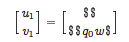
\includegraphics[scale=0.9]{tesi_stile/img/cap7f4.png}
\end{figure}\\
Per ogni quintupla $(q,a,r,b, +1)$ aggiungiamo la coppia\\
\begin{figure}[htp]
    \centering
    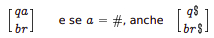
\includegraphics[scale=0.9]{tesi_stile/img/cap7f5.png}
\end{figure}\\
Per ogni quintupla $(q,a,r,b, -1)$ aggiungiamo le coppie\\
\begin{figure}[htp]
    \centering
    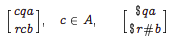
\includegraphics[scale=0.9]{tesi_stile/img/cap7f6.png}
\end{figure}\\
\newpage
Per ogni $a \in A$ U $\{\#,\$\}$, aggiungiamo la coppia\\
\begin{figure}[htp]
    \centering
    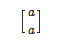
\includegraphics[scale=0.9]{tesi_stile/img/cap7f8.png}
\end{figure}\\
Infine aggiungeremo le coppie\\
\begin{figure}[htp]
    \centering
    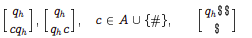
\includegraphics[scale=0.9]{tesi_stile/img/cap7f9.png}
\end{figure}\\
\textbf{Esempio}\\
Istruzioni:
\begin{center}
    $(q_0, 1, q_1, \#, +1), (q_0, \#, q_0, \#, +1), (q_1, 1, q_0, \#, +1), (q_1, \#, q_h , \#, +1)$
\end{center}
Input: w = 111\\
Istanza di MPCP:
\begin{figure}[htp]
    \centering
    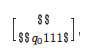
\includegraphics[scale=0.8]{tesi_stile/img/cap7f10.png}
    \includegraphics[scale=0.8]{tesi_stile/img/cap7f11.png}
    \includegraphics[scale=0.8]{tesi_stile/img/cap7f12.png}
\end{figure}\\
\begin{center}
    \textbf{Se M $\uparrow$ w non ci sono match !}
\end{center}
\newpage
\subsection{Ridurre MPCP a PCP}
\begin{figure}[htp]
    \centering
    \includegraphics[scale=0.9]{tesi_stile/img/cap7f13.png}
\end{figure}
Se invece M $\downarrow$ w, continuando, otterremo\\
\begin{figure}[htp]
    \centering
    \includegraphics[scale=0.9]{tesi_stile/img/cap7f14.png}
\end{figure}\\
\textbf{Asserto}\\
Si ha M $\downarrow$ w se e solo se $P_{M,w} \in$ MPCP.\\\\
\textbf{Corollario}\\
Il problema dell’arresto si riduce a MPCP.\\
Ora costruiamo una riduzione di MPCP a PCP. Per ogni parola $w =a_1a_2 ... a_l$, denotiamo:
\begin{center}
    $*w = *a_1 *a_2 ... *a_l$,  $w*=a_1* a_2* ... a_l*$
\end{center}
Dobbiamo costruire una funzione che a ogni istanza P di MPCP associ un'istanza P' di PCP, in modo tale che P ha un match con $i_1 = 1$ se e solo se P' ha un match.\\
Sia $P = (u_1, v_1; u_2, v_2;...;u_n,v_n)$. Definiamo\\
\begin{center}
   P' = $(*u_1,v_1*; *u_1, v_1*;*u_2, v_2*; ... , *u_n, v_n*; *o, o)$
\end{center}
\newpage
\begin{figure}[htp]
    \includegraphics[scale=0.9]{tesi_stile/img/cap7f16.png}
\end{figure}
Viceversa, se P ha un match con $i_1 = 1$, allora ci sarà anche un match di P'.
Se ne conclude che P' $\in$ PCP se e solo se P $\in$ MPCP.\\\\
\textbf{Conclusione}\\
Abbiamo costruito una riduzione del problema dell’arresto a MPCP e una riduzione di MPCP a PCP.\\
Poichè il problema dell’arresto è indecidibile, lo sono anche MPCP e PCP.
\subsection{Matrici con angolo zero in alto a destra}
\textbf{Problema (Zero nell’angolo)}\\
Dato un insieme finito M di matrici 3 x 3 a coefficienti interi, esiste un prodotto di matrici di M che ha uno 0 nell’angolo in alto a destra?.\\\\
\textbf{Teorema}\\
Il problema Zero nell’angolo è indecidibile.\\\\
\textbf{Dimostrazione}\\
PCP si riduce al problema Zero nell’angolo.
\newpage
\subsection{Riduzione di PCP a Zero nell’angolo}
Sia $P = (u_1,v_1;...;u_n,v_n)$ un’istanza di PCP.\\
Costruiremo un insieme di matrici M = $\{M_1,.., M_n\}$ tali che P $\in$ PCP.\\
se e solo se M contiene una matrice con zero nell’angolo in alto a destra. \\
Possiamo supporre, senza perdita di generalità, che l’alfabeto sia $\{1, 2, . . . , d - 1\}$.\\
Per $i=1, . . . , n$ definiamo:
\begin{figure}[htp]
    \centering
    \includegraphics[scale=0.9]{tesi_stile/img/cap7f17.png}
\end{figure}\\
dove $(w)_d$ è il numero denotato da w in base d. Si verifica facilmente che
\begin{figure}[htp]
    \centering
    \includegraphics[scale=0.9]{tesi_stile/img/cap7f18.png}
\end{figure}\\
$i_1, . . . , i_m \in \{1, . . . , n\}$.\\
Ma allora $M_{i1}...M_{im}$ ha zero nell’angolo in alto a destra se e solo se $(i_1, . . . , i_m )$ è un match di P.\\
Questo prova che la funzione $P \mapsto M$ è una riduzione di PCP a Zero nell’angolo.\\
Con tecniche simili, si dimostra l’indecidibilità del \textbf{problema di mortalità} per le matrici 3 x 3 a coefficienti interi:\\\\
\textbf{Problema (mortalità)}\\
Dato un insieme finito M di matrici 3 x 3 a coefficienti interi, esiste un prodotto di matrici di M uguale alla matrice nulla?
\newpage
\subsection{CFG ambigue}
\textbf{Definizione}\\
Una grammatica non contestuale è ambigua se esiste una parola con due derivazioni sinistre.\\\\
\textbf{Teorema}\\
È indecidibile se una grammatica non contestuale è ambigua.\\\\
\textbf{Dimostrazione}\\
PCP si riduce all’ambiguità delle grammatiche non contestuali.\\
Sia $P = (u_1,v_1; . . . ;u_n,v_n)$ un’istanza di PCP.\\
Costruiremo una grammatica non contestuale G che è ambigua se e solo se P $\in$ PCP.\\
Siano c1,..., cn n nuove lettere e G la grammatica con le produzioni\\
\begin{center}
    $ S \mapsto X$ | $Y, X \mapsto u_iX_{ci}$ | $uici, Y \mapsto v_iY_{ci}$ | $vici$, i = 1, . . . , n.
\end{center}
Si verifica facilmente che G genera il linguaggio:
\begin{figure}[htp]
    \centering
    \includegraphics[scale=0.9]{tesi_stile/img/cap7f20.png}
\end{figure}
Non è poi difficile convincersi che G è ambigua se e soltanto se
\begin{center}
    $u_{i1} ... u_{il} = v_{i1} ... v_{il}$
\end{center}
per opportuni $i_1, . . . , i_l$ cioè se e soltanto se P ha un match.
    \chapter{Funzioni ricorsive} \label{ch:capitolo8}
\subsection{Approcci alternativi alla nozione di calcolabilità}
\begin{itemize}
    \item Calcolo equazionale (Gödel,Herbrand,Kleene)
    
    \item lambda-calcolo (Church)
    
    \item funzioni ricorsive parziali (Gödel,Kleene)
    
    \item macchina di Turing
    
    \item sistemi di deduzioni canonici (Post)
    
    \item sistemu di Markov
    
    \item URM (Sheperdson, Sturgis)
\end{itemize}
\textbf{Terorema}\\
Ognuno dei metodi precedenti genera la medesima classe di funzioni
\newpage
\subsection{Funzioni ricorsive di base}
Nel seguito, considereremo esclusivamente funzioni (parziali o totali)
\begin{center}
    $f : N^k \mapsto N$
\end{center}
con $k >= 0$ (l’intero k si dice arietà di f ; nel caso k = 0, f è una costante).\\\\
\textbf{Definizione}\\
Chiameremo funzioni primitive di base le funzioni seguenti.
\begin{enumerate}
    \item La funzione \textbf{successore}
    \begin{center}
        $s$ : $N \mapsto N$ definita da $s(x) = x + 1$
    \end{center}
    \item La funzione \textbf{zero}
    \begin{center}
         $z$ : $N \mapsto N$ definita da $z(x) = 0$
    \end{center}
    \item Le \textbf{proiezioni} 
    \begin{center}
        $P^k_i $ : $N^k \mapsto N $ definita da $P^k_i(x_1,...,x_k) = x_i$ con $1 <= i <= k$
    \end{center}
\end{enumerate}
\subsection{Composizione e recursione}
\textbf{Definizione}\\
Siano $k, n > 0$ con , $h:$ $N^k \mapsto N$ e $g_1,...,g_n:$ $N^k \mapsto N$ funzioni totali.\\
La funzione $f:$ $N^k$ $\mapsto N$ definita da$:$
\begin{center}
    $f(x_1, ... , x_k )= h(g_1(x_1, ... , x_k), ... , g_n(x_1, ... ,x_k))$
\end{center}
si dice la funzione ottenuta per composizione dalle funzioni $h, g_1, ... , g_n$.\\\\
\textbf{Definizione}\\
Sia $k >= 0, h:$ $n^k+2 \mapsto N$ e $g : N^k \mapsto N$ funzioni totali.\\
La funzione $f:N^k+1 \mapsto N$ definita da
\begin{center}
    $f(x_1,..,x_k, 0) = g(x_1,...,x_k)$\\
    $f(x_1,..,x_k, y+1) = h(x_1,...,x_k, y, f(x_1,...,x_k, y)$\\
\end{center}
si dice la funzione ottenuta per \textbf{recursione} dalle funzioni g e h.
\subsection{Funzioni ricorsive primitive}
\textbf{Definizione}\\
Una funzione si dice ricorsiva primitiva se si può ottenere dalle funzioni ricorsive di base con un numero finito di operazioni di composizione e recursione.\\\\
\textbf{Osservazione}\\
Le funzioni ricorsive primitive sono Turing-calcolabili.\\\\
\textbf{Esempi}
\begin{figure}[htp]
    \includegraphics[scale=0.9]{tesi_stile/img/f1cap8.png}
\end{figure}
\newpage
\subsection{La funzione di Ackermann}
\textbf{Problema}\\
La nozione di funzione ricorsiva primitiva coincide con la nozione intuitiva di funzione calcolabile?
\begin{figure}[htp]
    \includegraphics[scale=0.9]{tesi_stile/img/f2cap8.png}
\end{figure}
La funzione $A(n, x) = x \uparrow^n x$ è la funzione di Ackermann.\\
\textbf{Osservazione}\\
\begin{itemize}
    \item La funzione di Ackermann è effettivamente calcolabile
    
    \item cresce molto velocemente
\end{itemize}
\textbf{Teorema}\\
Per ogni funzione ricorsiva primitiva f esiste |$x_0 >= 0$ tale che
\begin{center}
    $f (x) < A(x_1, x_1)$, per ogni $x >= x0$
\end{center}
\textbf{Corollario}\\
La funzione di Ackermann non è ricorsiva primitiva.
\newpage
\subsection{Minimalizzaione}
\textbf{Definizione}\\
Sia $k > 0$ e $g: N^k+1 \mapsto N$ una funzione totale. La funzione parziale $f:N^k \mapsto N$ definita da
\begin{center}
    $f(x_1, ... , x_k ) = min\{y$ | $g(x_1, .. , x_k, y) = 0\}$
\end{center}
si dice ottenuta da g per minimalizzazione.\\\\
\textbf{Osservazione}\\
Se g è calcolabile, allora lo è anche f.\\\\
\textbf{Osservazione}\\
Le nozioni di composizione e recursione si estendono naturalmente alle funzioni parziali.
\subsection{Composizione e recursione}
\textbf{Definizioni}\\
Sia $k > 0$ e $h: N^n \mapsto N$ una funzione ottenuta per composizione dalle funzioni $h_1, g_1,...,g_n$. avrà dominio
\begin{figure}[htp]
    \centering
    \includegraphics[scale=0.7]{tesi_stile/img/f4cap8.png}
\end{figure}\\
è definito da:
\begin{figure}[htp]
    \centering
    \includegraphics[scale=0.7]{tesi_stile/img/f5cap8.png}
\end{figure}\\
Sia $k >= 0$ , $h: N^{k+2} \mapsto N$ e $g: N^k \mapsto N$  funzioni parziali.\\
La funzione f ottenuta per recursione dalle funzioni g e h avrà dominio definito da
\begin{figure}[htp]
    \centering
    \includegraphics[scale=0.7]{tesi_stile/img/f6cap8.png}
\end{figure}\\
e sarà definito da:
\begin{figure}[htp]
    \centering
    \includegraphics[scale=0.7]{tesi_stile/img/f7cap8.png}
\end{figure}
\newpage
\subsection{Funzioni ricorsive parziali}
\textbf{Definizioni}\\
Una funzione si dice ricorsiva parziale se si può ottenere dalle funzioni
ricorsive di base con un numero finito di operazioni di composizione,
recursione e minimalizzazione.
Si dice funzione ricorsiva una funzione parziale ricorsiva che sia anche
totale.
Infine, un sottoinsieme di N si dice ricorsivo se la sua funzione
caratteristica è ricorsiva.\\\\
\textbf{Proposizione}\\
Le funzioni ricorsive parziali sono calcolabili.
\subsection{Funzioni ricorsive parziali e calcolabilità}
\textbf{Teorema}\\
Una funzione è ricorsiva parziale se e solo se è Turing-calcolabile.\\\\
\textbf{Corollario}\\
Un insieme è ricorsivo se e solo se è decidibile.\\
Diremo che un insieme è ricorsivamente enumerabile se è vuoto o è l’immagine di una funzione ricorsiva.\\\\
\textbf{Corollario}\\
Un insieme è ricorsivamente enumerabile se e solo se è semidecidibile.
\newpage
\subsection{Dimostrazione}
Si è già visto che le funzioni ricorsive parziali sono Turing-calcolabili.
Dobbiamo provare che le funzioni Turing-calcolabili sono ricorsive parziali.
Sia quindi $f$ una funzione Turing-calcolabile e sia $M$ la macchina di Turing che la calcola.
Per ogni descrizione istantanea $C$ di $M$, denoteremo con $gn(C)$ il suo numero di Gödel.\\
Consideriamo le funzioni
\begin{figure}[htp]
    \includegraphics[scale=0.9]{tesi_stile/img/f3cap8.png}
\end{figure}
\newpage
\subsection{Dimostrazione-2}
Le funzioni start, next, tape sono ricorsive primitive. Definiamo $g:N^2 \mapsto N$ con
\begin{center}
    $g(x_1,0) = start(x), g(x ,t+1) = next(g(x_1 ,t)).$
\end{center}
La funzione g calcola il numero di Gödel della configurazione istantanea di M su input x dopo t passi.\\
E' ricorsiva primitiva.\\
La funzione\\
\begin{center}
    $h(x) = min \{t | g(x ,t) = 0\}$
\end{center}
calcola il numero di passi in cui M si arresta su input x , diminuito di 1; è ricorsiva parziale.\\
La funzione\\
\begin{center}
    $k(x) = tape(pred(h(x)$
\end{center}
calcola l’output di $M$ su input x, cioè $f(x)$; è ricorsiva parziale.

    \chapter{Teoria della complessità} \label{ch:capitolo9}
\subsection{Costo della computazione}
\textbf{Problema}\\
Cosa si può calcolare con un costo ragionevole?\\\\
\textbf{Osservazione}\\
Il costo dipende dall’algoritmo\\\\
\textbf{Esempio}\\
Vogliamo determinare il valore del polinomio
\begin{center}
    $x^7 + 5x^6 + 2x^4 + 12x^3 + 5x^2 + 2x + 21$
\end{center}
per certi input x . Quante moltiplicazioni servono?
\begin{itemize}
    \item per ciascun monomio, nell’ordine, 6,6,4,3,2,1, totale: 22
    
    \item se calcolo prima tute le potenze di x (6 moltiplicazioni), per ciascun monomio, nell’ordine, 0,1,1,1,1,1, totale: 11
    
    \item se scrivo il polinomio nella forma
\end{itemize}
\begin{center}
    $(((((x + 5)x^2 + 2)x + 12)x + 5)x + 2)x + 21$
\end{center}
\newpage
\textbf{Esempio}\\
Per calcolare il massimo comun divisore di due interi positivi a e b si può:
\begin{itemize}
    \item decomporre a e b in fattori primi
    
    \item selezionare i fattori primi comuni, con il minimo esponente
\end{itemize}
oppure usare l’algoritmo di Euclide:\\
\begin{figure}[htp]
    \centering
    \includegraphics[scale=0.9]{tesi_stile/img/f1cap9.png}
\end{figure}
\newpage
\begin{figure}[htp]
    \centering
    \includegraphics[scale=0.9]{tesi_stile/img/f2cap9.png}
\end{figure}
Per risolvere un sistema lineare si può utilizzare il metodo di Cramer:\\
\begin{figure}[htp]
    \centering
    \includegraphics[scale=0.9]{tesi_stile/img/f3cap9.png}
\end{figure}\\
oppure ridurre il sistema in forma triangolare:\\
\begin{figure}[htp]
    \centering
    \includegraphics[scale=0.9]{tesi_stile/img/f4cap9.png}
\end{figure}
\newpage
\subsection{Teoria della complessità}
\textbf{Quale risorsa misurare?}\\
Tempo, memoria, energia,...\\\\
\textbf{Quale modello di calcolo?}\\
Macchina di Turing, altri?.\\\\
\textbf{Quali problemi considerare?}\\
\begin{itemize}
    \item Problemi di \textbf{decisione}
    
dato $S \subseteq A*$, decidere per ogni input $w \in A*$ se $w \in S$.

    \item Problemi di \textbf{computazione}
    
Data $f : A* \mapsto A*$ calcolare, per ogni input $w \in A*$ , f(w)

    \item problemi di ottimizzazione
    
    \item problemi di ricerca

\end{itemize}
\subsection{Teoria della complessità2}
\textbf{Che risultati cerchiamo?}\\
Vogliamo conoscere il costo minimo per risolvere un problema (non un particolare algoritmo). Ci aspettiamo
\begin{itemize}
    \item Risultati negativi
    
    il problema non si può risolvere senza...
    
    \item Risultati di confronto
    
    per risolvere il problema S servono almeno le stesse risorse necessarie a risolvere il problema T
\end{itemize}
\subsection{Come misurare la complessità}
Vogliamo valutare il costo della computazione in funzione della complessità dell’input.
Sia S un problema (di decisione) sull’alfabeto A. Consideriamo una funzione $f : N \mapsto N$ calcolata come segue:
\begin{itemize}
    \item per ogni $n \in N$ consideriamo tutti gli input di lunghezza minore o uguale a n e il costo delle relative computazioni (escludendo quelle che non terminano)
    
    \item f(n) restituirà il massimo costo di tali computazioni
\end{itemize}
\textbf{Proprietà delle funzioni costo}
\begin{itemize}
    \item una funzione costo è definita per n $>= n_0$, con $n_0 \in N$ opportuno
    
    \item non decrescente
    
    \item non limitata
\end{itemize}
\textbf{Esempi}\\
$n, n^2, n^k, 2^n, 2^{2n}, |\log_2 n|$, polinomi a coefficienti non negativi.\\\\
\newpage
\textbf{Esempio}\\
Quante divisioni servono per l’algoritmo Euclideo del MCD?\\
Supponiamo a $>=$ b e calcoliamo MCD(a, b).\\
\begin{figure}[htp]
    \centering
    \includegraphics[scale=0.9]{tesi_stile/img/f5cap9.png}
\end{figure}\\
Pertanto.
\begin{figure}[htp]
    \includegraphics[scale=0.9]{tesi_stile/img/f6cap9.png}
\end{figure}\\
Ne segue\\
\begin{center}
    $k < 2\log_2 a$
\end{center}
Pertanto:\\
Il numero di divisioni necessario per calcolare MCD(a, b) è linearmente limitato dalla lunghezza della rappresentazione binaria di a.\\\\
\textbf{Osservazione}\\
Per le funzioni numeriche, la complessità dell’input è misurata dal numero di bit (o cifre decimali) necessaria per rappresentarlo:
\begin{center}
    $1 + |\log_2(n)|$
\end{center}
\newpage
\subsection{Complessità temporale}
\textbf{Definizione}\\
Sia M una macchina di Turing. Si dice complessità temporale di M la funzione $c_M : N \mapsto N$ definita come segue:\\
per ogni $n \in N$, $c_M (n)$ è il massimo numero di passi di una computazione convergente di M su un input di lunghezza minore o uguale a n.\\\\
\textbf{Osservazione}\\
La funzione $c_M$ è definita per $n >= n_0$ con $n_0 \in N$, non decrescente e non limitata (purchè $c_M$ abbia un dominio infinito e M esamini l’intero input su ogni computazione).
\subsection{La classe P}
\textbf{Definizione}\\
Denotiamo con P la classe dei problemi S accettati da una macchina di Turing M tale che $c_M (n) = O(n^k)$ per qualche intero positivo k.\\\\
\textbf{Osservazione}\\
Se $S \in P$, allora c’è una macchina di Turing che, per ogni input w di lunghezza n, si comporta nel modo seguente:
\begin{itemize}
    \item se $w \in S$, allora M accetta w in al più $cl(w)^k$ passi (con c, k costanti positive fissate)
    
    \item se $w \notin S$, allora $M \uparrow w$
\end{itemize}
In realtà, c’è anche una macchina di Turing M'
che decide S con $c_{M'}(n) = O(n^k)$.
\newpage
\subsection{Tesi di Edmonds-Cook-Karp}
\begin{figure}[htp]
    \centering
    \includegraphics[scale=0.9]{tesi_stile/img/f10cap9.png}
\end{figure}
\textbf{Osservazione}\\
Riferita ai problemi, non agli algoritmi.\\\\
\textbf{Osservazione}\\
La definizione di P è robusta:\\
se esiste un algoritmo che decide S e richiede l’esecuzione di $O(n^k)$ istruzioni (comunque specificate, purchè simulabili da una macchina di Turing in tempo polinomiale), allora $s \in P$.





    \chapter{La classe P} \label{ch:capitolo10}
\subsection{La classe P}
\textbf{Definizione}\\
Denotiamo con P la classe dei problemi S accettati da una macchina di Turing M tale che $c_M (n) = O(n^k)$ per qualche intero positivo k.\\\\
\textbf{Osservazione}\\
Se $S \in P$, allora c’è una macchina di Turing che, per ogni input w di lunghezza n, si comporta nel modo seguente:
\begin{itemize}
    \item se $w \in S$, allora M accetta w in al più $cl(w)^k$ passi (con c, k costanti positive fissate)
    
    \item se $w \notin S$, allora M $\uparrow$ w
\end{itemize}
In realtà, c’è anche una macchina di Turing M' che decide S con $c_M'(n) = O(n^k)$.
\subsection{2Col}
\textbf{Definizione}\\
Un grafo $G = (V , E)$ è 2-colorabile se esiste una funzione $c : V \mapsto \{1, 2\}$ tale che per ogni $(v, w) \in E$, $f(v) \neq f (w)$.\\
La classe dei grafi 2-colorabili è denotata 2COL.\\\\
\textbf{Proposizione}\\
2COL $\in$ P.\\\\
\textbf{Dimostrazione}\\
È sufficiente trovare un algoritmo che risolve 2COL in tempo polinomiale.\\
\begin{figure}[htp]
    \centering
    \includegraphics[scale=0.9]{tesi_stile/img/foto1cap10.png}
\end{figure}
\subsection{Algoritmo}
Su input G.
\begin{figure}[htp]
    \includegraphics[scale=0.9]{tesi_stile/img/foto2cap10.png}
\end{figure}
\subsection{SAT}
Siano $x_0, x_1, x_2,...$una famiglia, potenzialmente infinita di variabili. Chiameremo letterali le variabili $x_i$ e le loro negazioni $\bar{x}_i$. Una clausola è una sequenza di letterali che non contiene letterali col
medesimo indice.\\
Un sistema di clausole si dice soddisfacibile se esiste una clausola che le interseca tutte (ossia contiene un letterale di ogni clausola del sistema) La famiglia dei sistemi di clausole soddisfacibili è denotata con SAT.\\\\
\textbf{Esempio}\\
Il sistema.
\begin{center}
    $\{(x_0 + \bar{x}_1)(x_0 + \bar{x}_1 + x_2)(x_3 + x_4 + \bar{x}_0)(\bar{x}_4 + \bar{x}_5)\}$
\end{center}
Una clausola che soddisfa il sistema non è altro che un implicante dell’espressione medesima.
Quindi un sistema è soddisfacibile se la corrispondente espressione Booleana non è nulla.
\subsection{2SAT}
\textbf{Definizione}\\
Una clausola di lunghezza 2 si dice 2-clausola.\\
L’insieme dei sistemi di 2-clausole soddisfacibili si denota con 2SAT.\\
\textbf{Proposizione}\\
2SAT $\in$ P.\\\\
\textbf{Dimostrazione}\\
Dobbiamo trovare un algoritmo che risolve 2SAT in tempo polinomiale.\\\\
\textbf{Esempio}\\
\begin{figure}[htp]
    \centering
    \includegraphics[scale=0.9]{tesi_stile/img/foto3cap10.png}
\end{figure}
\newpage
\subsection{Ridurre 2COL a 2SAT}
Costruiamo una riduzione di 2COL a 2SAT.\\
Devo costruire una funzione calcolabile totale f che a ogni grafo G associa un sistema di 2-clausole f (G) tale che.\\
foto.\\
Sia G = (V , E) un grafo.\\
Per ogni vertice $v_i,i = 1, . . . , n$, introduco una variabile $x_i$ ($x_i$ = "$v_i$ ha colore verde") e per ogni lato $(v_i, v_j) \in E$, le due clausole
\begin{center}
    $x_i, x_j, \bar{x}_i, \bar{x}_j$
\end{center}
(uno dei vertici ha colore verde, uno non ha colore verde).\\\\
\textbf{Algoritmo alternativo per 2COL}\\
Su input G
\begin{figure}[htp]
    \includegraphics[scale=0.9]{tesi_stile/img/foto4cap10.png}
\end{figure}
\newpage
\subsection{Equazioni lineari}
\textbf{Probelma}\\
\textbf{Input}: Un'equazione $ax + by = c$ con $a, b, c \in Z$
\\\textbf{Output}: si se l’equazione ha una soluzione intera, no altrimenti.\\\\
\textbf{Osservazione}
\begin{itemize}
    \item Se MCD(a, b) = 1, l’equazione ha soluzione intera (teorema di Bezout)
    
    \item Se MCD(a, b) divide c, ci si può ricondurre al caso precedente
    
    \item Se l’equazione ha una soluzione intera, allora MCD(a, b) divide c.
    
\end{itemize}
\textbf{Soluzione}\\
Per risolvere il problema basta calcolare MCD(a, b) e verificare se divide c.\\
Sono necessarie
\begin{itemize}
    \item $O(n^2)$ divisioni, n = $\log_2$ (max$\{a, b, c\}$)
    
    \item Per ogni divisione, $O(n)$ sottrazioni
    
    \item Per ogni sottrazione $O(n)$ operazioni elementari sui bit.
    
    \item totale: $O(n^4)$ operazioni elementari: il problema è nella classe P
\end{itemize}
\newpage
\subsection{Numeri primi}
\textbf{Problema}\\
\textbf{Input:} Un numero a $\in$ N.\\
\textbf{Output:} Si se a è primo, no altrimenti.\\\\
\textbf{Soluzione}\\
Dividi a per tutti gli interi $q = 2, 3,..,|\sqrt{a}|$.
\begin{itemize}
    \item ma sono $|\sqrt{a} - 1| =$ $O(2^{n/2})$ divisioni, $n = \log_2$a
\end{itemize}
L’algoritmo di Agrawal, Kayal, Saxena (2002), ha complessità $O(n^11)$.
Quindi il problema è nella classe P.\\\\
\textbf{Osservazione}\\
Nella pratica, la complessità $n^11$ è troppo alta, per cui per la ricerca di grandi primi si preferiscono algoritmi probabilistici.\\\\
\textbf{Problema}
\textbf{Input:} Un numero $a \in N$.\\
\textbf{Output:} la decomposizione di a in fattori primi.
\subsection{coP}
\textbf{Definizione}\\
Denotiamo coP la classe dei problemi il cui complemento è in P.\\\\
\textbf{Proposizione}\\
coP = P.\\\\
\textbf{Dimostrazione}\\
Se $S \in coP$, c’è una macchina di Turing M che decide S con $c_M(n) = O(n^k)$, per k opportuno.\\
Ma allora c’è una macchina M' che accetta S, con $c_M'(n) = c_M(n) = O(n^k)$\\


(basta aggiungere le istruzioni affinchè M con output SI inizi un loop infinito).




    \chapter{La classe NP} \label{ch:capitolo11}
\subsection{Macchine di Turing non deterministiche}
Una Macchina di Turing M è una quadrupla $(Q, A, \sigma, q_0)$, dove:
\begin{itemize}
    \item Q è un insieme finito di stati
    
    \item A è un alfabeto, cui si aggiunge il simbolo bianco \#
    
    \item $\sigma$ è una funzione da Q × (A U $\{\#\}$) a p(Q × (A U $\{\#\}$) × $\{-1, +1\}$), chiamata funzione di transizione
    
    \item $q_0 \in Q$ è lo stato iniziale
\end{itemize}
Le quintuple (q, a, q', a', x ) tali che (q', a', x) $\in \sigma(q, a)$ sono dette le istruzioni di M.
\subsection{Configurazioni consecutive}
\textbf{Definizione}\\
Una configurazione istantanea di una Macchina di Turing M = (Q, A, $\sigma$, $q_0$) è un elemento dell’insieme (A U $\{\#\}$)$^*$ x Q x (A U $\{\#\}$) x (A U $\{\#\}^*$.
Nell’insieme delle configurazioni istantanee di M introduciamo la relazione binaria $\vdash_M$ che associa alla configurazione C quelle che possono seguirla in una computazione di M. Qualora non esistesse nessuna configurazione di questo tipo, scriveremo $C\vdash/_M$\\\\
\textbf{Esempio}\\
Se M ha l’istruzione (q, a, q', b, $-1$) e (q, a, q'', a, $+1$), allora.\\
\begin{figure}[htp]
    \includegraphics[scale=0.9]{tesi_stile/img/foto1cap11.png}
\end{figure}
\subsection{Computazioni}
\textbf{Definizioni}\\
\begin{itemize}
    \item La configurazione iniziale C0 di una macchina di Turing non deterministica M sull’input w è definita come nel caso deterministico,
    
    \item una sequenza
    
    $C_0\vdash_M$, $C_1\vdash_M$ ... $C_n\vdash/_M$
    
    si dirà una computazione convergente di M sull’input w.
    
    \item Diremo che M accetta w se esiste una computazione convergente di M sull’input w.
\end{itemize}
\textbf{Osservazione}\\
Quindi M accetta w se almeno una computazione di M su w converge, M rifiuta w se tutte le computazioni di M su w divergono.
\subsection{Complessità temporale per macchine di Turing non deterministiche}
\textbf{Definizione}\\
Sia M una macchina di Turing non deterministica.
Per ogni parola w accettata da M, denotiamo con $t_w$ il minimo numero di passi di una computazione convergente di M su input w.
Si dice complessità temporale di M la funzione $c_M : N \mapsto N$ definita come segue: per ogni $n \in N$
\begin{center}
    $c_M (n)$ = max$\{t_w | w accettata da M_1, l(w) <= n\}$.
\end{center}
\textbf{Osservazione}\\
Ovviamente, una macchina di Turing deterministica si può considerare come una particolare macchina di Turing non deterministica in cui, per ogni input, c’è un’unica computazione. \\
In tal caso, la definizione di $c_M (n)$ coincide con quella già data in precedenza.
\subsection{Macchine e linguaggi}
\textbf{Definizione}\\
L’insieme delle parole accettate da una macchina di Turing non deterministica M si dirà il linguaggio accettato da M.\\\\
\textbf{Proposizione}\\
I problemi accettati da macchine di Turing non deterministiche sono semi-decidibili.\\\\
\textbf{Dimostrazione}\\
Una macchina di Turing deterministica può simulare, parallelamente, le computazioni di una macchina di Turing non deterministica su un dato
input.\\
Tale macchina accetterà se almeno una delle computazioni della macchina
non deterministica termina.
\subsection{La classe NP}
\textbf{Definizione}\\
Denotiamo con NP la classe dei problemi S accettati da una macchina di Turing non deterministica M tale che $c_M(n) = O(n^k)$ per qualche intero positivo k.\\\\
\textbf{Osservazione}\\
Se $S \in NP$, allora ci sono una macchina di Turing non deterministica M, e due interi positivi c e k tali che, per ogni input w di lunghezza n, M si comporta nel modo seguente:
\begin{itemize}

    \item se $w \in S$, allora esiste almeno una computazione convergente M su w con al più c l(w) k passi
    
    \item se $w \notin S$, allora tutte le computazioni di M su w divergono.
\end{itemize}
\textbf{Osservazione}\\
Riferita ai problemi, non agli algoritmi.\\\\
\textbf{Osservazione}\\
Come quella di P, anche la definizione di NP è robusta:\\
se esiste una procedura non deterministica che accetta le parole di S e richiede l’esecuzione di $O(n^k)$ istruzioni (comunque specificate, purchè simulabili da una macchina di Turing in tempo polinomiale), allora $S \in NP$.
\subsection{SAT}
Il problema SAT è accettato dalla seguente procedura non-deterministica:\\
Dato un sitema di clausole S
\begin{enumerate}
    \item assegna (non deterministicamente) dei valori di verità alle variabili
    
    \item se tutte le clausole sono soddisfatte accetta, altrimenti divergi
\end{enumerate}
Ciascuna esecuzione del primo passo richiede tempo lineare (in termini di operazioni elementari)\\
Il secondo passo si può eseguire in tempo quadratico.
\begin{center}
    \textbf{SAT $\in$ NP}
\end{center}
\textbf{Osservazione}\\
Il passo 1 può essere eseguito in $2^k$ modi diversi, dove k è il numero delle variabili.
\subsection{3COL}
Il problema 3COL è accettato dalla seguente procedura non-deterministica:\\
Dato un grafo G
\begin{enumerate}
    \item  assegna (non deterministicamente) dei colori ai vertici
    
    \item  verifica se, per ogni lato, i vertici agli estremi hanno colore diverso
    
    \item in caso affermativo accetta, altrimenti divergi.
\end{enumerate}
Ciascuna esecuzione del primo passo richiede tempo lineare (in termini di operazioni elementari, rispetto al numero dei vertici)\\
Il secondo passo si può eseguire in tempo quadratico.
\begin{center}
    \textbf{3COL $\in$ NP}
\end{center}
\textbf{Osservazione}\\
Il passo 1 può essere eseguito in $3^k$ modi diversi, dove k è il numero dei vertici.
\subsection{Grafi}
Sia G = (V,E) un grafo e $V_0 \subseteq V$\\
L'insieme $V_0$ è indipendente se per ogni v, $v' \in V_0$, $(v, v') \notin E$.\\
L'insieme $V_0$ è una clique se per ogni v, v' $\in$ $V_0$, (v, v') $\in$ E.\\
L’insieme $V_0$ è un ricoprimento di vertici se per ogni (v, v') $\in$ E almeno uno dei vertici v,v' sta in $V_0$.\\\\
\textbf{Problema IS}\\
\textbf{Input:} Un grafo G = (V ,E) e un intero $k > 0$\\
\textbf{Output:} si se G ha un insieme\\ indipendente di ordine k, no altrimenti.\\\\
\textbf{Problema CLIQUE}\\
\textbf{Input:} Un grafo G=(V,E) e un intero $k > 0$\\
\textbf{Output:} si se G ha una clique di ordine k, no altrimenti.\\\\
\textbf{Problema VC}\\
\textbf{Input:} Un grafo G = (V,E) e un intero $k > 0$\\
\textbf{Output:} si se G ha un ricoprimento di vertici di ordine k, no altrimenti.
\subsection{Grafi-2}
\textbf{Proposizione}\\
Sia G = (V , E) un grafo e $V_0 \subseteq V$\\
Le seguenti condizioni sono equivalenti:
\begin{enumerate}
    \item $V_0$ è indipendente,
    
    \item $V_0$ è una clique del grafo complementare $\Bar{G} = (V , \Bar{E})$
    
    \item V / $V_0$ è un ricoprimento di vertici.
\end{enumerate}
\textbf{Corollario}\\
Ognuno dei problemi IS, CLIQUE e VC si riduce agli altri due.\\
Inoltre la funzione di riduzione si calcola rapidamente.\\\\
\textbf{Dimostrazione}\\
Sia G un grafo di ordine n. Allora.\\
\begin{figure}[htp]
    \includegraphics[scale=0.9]{tesi_stile/img/foto2cap11.png}
\end{figure}\\
\textbf{Osservazione}\\
I sottoinsiemi di V di ordine k sono 
$
\begin{pmatrix}
& n & \\
& k &
\end{pmatrix}	
$
e quindi non polinomialmente limitati da n (se k non è fissato).
\subsection{Grafi-3}
Il problema IS è accettato dalla seguente procedura non-deterministica:\\
Dato un grafo G e un intero $k > 0$.
\begin{enumerate}
    \item seleziona (non deterministicamente) k vertici
    
    \item verifica se, per ogni coppia di vertici selezionati v, v', (v, v') $\notin$ E
    
    \item in caso affermativo accetta, altrimenti divergi.
\end{enumerate}
Ciascuna esecuzione del primo passo richiede tempo polinomiale (in termini di operazioni elementari, rispetto al numero dei vertici) come pure il secondo passo.\\
In maniera simile, si trovano procedure non-deterministiche che accettano CLIQUE e VC, con la medesima complessità:
\begin{center}
    \textbf{IS, CLIQUE, VC $\in$ NP}
\end{center}
\subsection{coNP}
\textbf{Definizione}\\
coNP è la classe dei problemi il cui complemento sta nella classe NP.\\\\
\textbf{Osservazione}\\
Mentre P = coP, non è noto se NP = coNP.\\\\
\textbf{Proposizione}\\
$P \subseteq NP \cap coNP$
\subsection{Un'altra definizione di Np}
\textbf{Proposizione}\\
Sia $S \subseteq A^*$ un problema. Le seguenti condizioni sono equivalenti
\begin{enumerate}
    \item Esistono una macchina di Turing non deterministica M e un intero $k > 0$ tali che M accetta S e $c_M (n) = O(n^k)$
    
    \item Esistono un problema $T \subseteq A^* x B^*$ e un polinomio p(n) tali che $T \in P$ e per ogni $w \in A^*$
\end{enumerate}
\begin{figure}[htp]
    \centering
    \includegraphics[scale=0.9]{tesi_stile/img/foto3cap11.png}
\end{figure}
\textbf{Osservazione}\\
In altri termini, ogni problema di classe NP  sull’alfabeto A si ottiene da un sottoinsieme di classe P di $A^* x B^*$ con le due operazioni seguenti:
\begin{enumerate}
    \item Si scartano le coppie (w, y) con y' molto più lungo di w
    
    \item si proietta su $A^*$
\end{enumerate}
Sia S un problema che verifica la condizione 2\\
Per ogni $w \in S$, ci sarà una parola y tale che $(w, y) \in T$ e $l(y) <= p(l(w)$).\\
Chiameremo y il testimone (o soluzione) di w.\\
\newpage
\subsection{Il testimone}
Sia S un problema che verifica la condizione 2.\\
Per ogni $w \in S$, ci sarà una parola y tale che (w, y) $\in$ T e l(y)$ <= $p(l(w)).
Chiameremo y il testimone (o soluzione) di w.\\\\
\textbf{Osservazione}\\
La limitazione l(y)$ <= $ p(l(w)) serve ad assicurare che la condizione
(w, y) $\in$ T possa essere accertata in tempo polinomiale rispetto a l(w).
Invero, T è accettato da una macchina di Turing deterministica M tale che
$c_M(n) <= q_1(n)$, per un opportuno polinomio a coefficienti non negativi $q_1$.
Sia $q_2(n) = q_1(n + (p(n)))$. Se
\begin{center}
   (w, y) $\in$ T, l(y) $<=$ p(l(w)),
\end{center}
Allora M converge su (w, y) in al più $q_1(l(w) + l(y)) <= q_2(l(w)$) passi.\\\\
\textbf{Esempi}
\begin{figure}[htp]
    \includegraphics[scale=0.9]{tesi_stile/img/foto4cap11.png}
\end{figure}
\newpage
\subsection{Dimostrazione}
\begin{figure}[htp]
    \includegraphics[scale=0.9]{tesi_stile/img/foto5cap11.png}
\end{figure}
Esistono una macchina di Turing non deterministica M e un polinomio q(n) tali che M accetta S e $c_M (n) <= q(n)$.\\
Poniamo p(n) = q(n)(n + q(n) + 2).\\
Ogni $w \in S$ ha una computazione convergente con non più di q(l(w)) passi.\\
Tale computazione è descritta da una parola di lunghezza al più p(l(w)).\\
Poniamo\\
\begin{center}
    \item T = \{(w, y) | y computazione convergente di M su input w\}
\end{center}
Si ha $T \in P$ e\\
\begin{figure}[htp]
    \centering
    \includegraphics[scale=0.9]{tesi_stile/img/foto6cap11.png}
\end{figure}
\begin{figure}[htp]
    \includegraphics[scale=0.9]{tesi_stile/img/foto7cap11.png}
\end{figure}\\
Esistono un problema $T \in P$ e un polinomio p(n) tali che
\begin{figure}[htp]
    \centering
    \includegraphics[scale=0.9]{tesi_stile/img/foto10cap11.png}
\end{figure}
Il problema S è accettato dalla seguente procedura non-deterministica:\\
Dato w
\begin{enumerate}
    \item genera (non deterministicamente) y tale che $l(y)<= p(l(w))$
    
    \item verifica se (w, y) $\in$ T
    
    \item in caso affermativo accetta, altrimenti divergi
\end{enumerate}
Ciascuna esecuzione del primo passo richiede tempo polinomiale rispetto alla lunghezza di w.\\
L’esecuzione del secondo passo richiede tempo polinomiale rispetto alla
lunghezza di (w, y), che è maggiorata da $l(w) + p(l(w))$.\\
Quindi l’esecuzione del secondo passo richiede tempo polinomiale rispetto
alla lunghezza di w.






    \chapter{NP-completezza} \label{ch:capitolo12}
\subsection{P = NP?}
\begin{itemize}
    \item\textbf{P} 
    
è la classe dei problemi che ammettono un algoritmo di decisione rapido (= polinomiale)
    
    \item\textbf{NP} 
    
è la classe dei problemi che ammettono un algoritmo di verifica rapido (= polinomiale)
\end{itemize}
Quindi P $\subseteq$ NP significa la verifica è più rapida della decisione.\\
Ma P = NP significherebbe che se c’è una procedura rapida di verifica per S, ce n’è una di decisione, veloce anch’essa. 
\begin{itemize}
    \item P è la classe dei problemi accettati da macchine di Turing deterministiche in tempo polinomiale
    
    \item NP è la classe dei problemi accettati da macchine di Turing non deterministiche in tempo polinomiale
\end{itemize}
Ogni macchina di Turing non deterministica è simulata da una macchina di Turing deterministica, ma la complessità cresce esponenzialmente. Si può fare meglio?\\\\\\
\textbf{Osservazione}\\
Se trovo un problema S di classe NP che non sta in P, allora P $\neq$ NP, Per dimostrare P = NP, dovrei dimostrare che tutti i problemi S $\in$ NP sono di classe P.
Vedremo invece che esiste una famiglia di problemi di classe NP (tra i quali, p.es., SAT) tale che se anche uno solo di essi appartiene a P, allora P = NP.
\subsection{Riduzioni polinomiali}
\textbf{Definizione}\\
Siano S, T due problemi su alfabeti A, B, rispettivamente.\\
Una riduzione polinomiale di S a T è una funzione totale $f : A^* \mapsto B^*$ tale che
\begin{figure}[htp]
    \centering
    \includegraphics[scale=0.9]{tesi_stile/img/foto1cap12.png}
\end{figure}
calcolata da una macchina di Turing deterministica con complessità temporale polinomiale.
Se esiste una riduzione polinomiale di S a T, scriveremo $S <=_p T$.\\\\
\textbf{Osservazione}\\
La relazione $<=_p$ è riflessiva e transitiva (pre-ordine).\\\\
\textbf{Esempio}\\
2COL $<=_p$ 2SAT, IS $<=_p$ CLIQUE $<=_p$ VC $<=_p$ IS.\\\\
\textbf{Proposizione}\\
Siano S, T due problemi. Se S $<=_p$ T e T $\in$ P (risp., T $\in$ NP), allora S $\in$ P (risp., S $\in$ NP).
\newpage
\subsection{Problemi NP-ardui}
\textbf{Definizione}\\
Un problema T si dice NP-arduo se, per ogni S $\in$ NP si ha S $<=_p$ T.
Un problema T si dice NP-completo se è NP-arduo e appartiene alla classe
NP.\\\\
\textbf{Proposizione}\\
Sia S un problema NP-completo. Se S $\in$ P, allora P = NP.
\subsection{Un problema NP-completo}
Si consideri il seguente problema LHalt:\\\\
\textbf{Input:} una macchina di Turing non deterministica M, un input w di
M, un’altra parola u;\\
\textbf{Output:} SI se una computazione di M converge su w in al più l(u) passi, NO altrimenti.\\\\
\textbf{Proposizione}\\
Si ha LHalt $\in$ NP.\\\\
\textbf{Dimostrazione}\\
Il problema è accettato dalla seguente procedura non deterministica in
tempo polinomiale:
\begin{enumerate}
    \item calcolare k = l(u)
    
    \item eseguire (non deterministicamente) M su w per un massimo di k passi; se M non si arresta, proseguire con un ciclo infinito.
\end{enumerate}
\textbf{Proposizione}\\
Il problema LHalt è NP-arduo\\\\
\textbf{Dimostrazione}\\
Sia S $\in$ NP. Allora esiste una macchina di Turing non deterministica M che accetta S e tale che
\begin{center}
    $c_M(n) <= P(n)$
\end{center}
per un opportuno polinomio P. La funzione f definita da
\begin{figure}[htp]
    \centering
    \includegraphics[scale=0.9]{tesi_stile/img/foto2cap12.png}
\end{figure}
è una riduzione polinomiale di S a LHalt.\\
Data l’arbitrarietà di S, possiamo concludere che LHalt è NP-arduo.
Dalle proprietà precedenti segue immediatamente che\\\\
\textbf{Corollario}\\
LHalt è NP-completo.
\subsection{Il teorema di Cook-Levin}
\textbf{Teorema (Cook-Levin, 1971)}\\
SAT è NP-completo.\\\\
\textbf{Proposizione}\\
Si ha SAT $\in$ NP.\\\\
\textbf{Dimostrazione}\\
L’insieme
\begin{figure}[htp]
    \centering
    \includegraphics[scale=0.9]{tesi_stile/img/foto3cap12.png}
\end{figure}
è di classe P e si ha S $\in$ SAT $\Longleftrightarrow$(S,V) $\in$ SATsol per un opportuno V.
\newpage
\textbf{Proposizione}\\
SAT è NP-arduo.\\\\
\textbf{Dimostrazione}\\
Sia S $\in$ NP. Allora esiste una macchina di Turing non deterministica M che
\begin{center}
    $c_M(n) <= p(n)$
\end{center}
per un opportuno polinomio p.
Costruiremo una riduzione polinomiale di S a SAT.
\newpage
\section{Il Teorema di Cook-Levin - Approfondito}
Si consideri il seguente problema LHalt:\\
\textbf{INPUT:} una macchina di Turing non deterministica M, un input w di M, un’altra parola u;\\
\textbf{OUTPUT:} SI se M converge su w in al più l(u) passi, NO altrimenti.\\
Vedremo che LHalt è un problema NP-completo.\\\\
\textbf{Proposizione 1}\\ 
Si ha LHalt $\in$ NP.\\\\
\textbf{DIMOSTRAZIONE}\\ 
Una procedura non deterministica che accetta LHalt in tempo polinomiale è la seguente:
\begin{enumerate}
    \item calcolare k = l(u)
    \item eseguire (non deterministicamente) M su w per un massimo di k passi; se M non si arresta, proseguire con un ciclo infinito.
\end{enumerate}
Chiaramente, si ha (M, w, u) $\in$ LHalt se e solo se una delle possibili esecuzioni della suddetta procedura termina. \\Poiché la simulazione è limitata a k = l(u) passi, la classe di complessità è NP.\\
\\\textbf{Proposizione 2}
\\Il problema LHalt è \textbf{NP-arduo.}
\\\textbf{DIMOSTRAZIONE} 
\\Sia S $\in$ NP. Allora esiste una macchina di Turing non deterministica M che accetta S e tale che 
\begin{center}
    $c_M(n) <= P(n)$
\end{center}
per un opportuno polinomio P. La funzione f definita da:
\begin{center}
    $w  \mapsto , w, 1^{P(l(w)})$
\end{center}
è una riduzione di S a LHalt. Il calcolo di tale funzione si riduce al calcolo di $k = P(l(w))$ e alla concatenazione di M, w e $1^k$. Si calcola pertanto in tempo costante. Data l’arbitrarietà di S, possiamo concludere che ogni problema di classe NP si riduce a LHalt in tempo polinomiale (anzi, costante). Questo dimostra che LHalt è
NP-arduo.
\\Dalle proprietà precedenti segue immediatamente che\\\\
\textbf{Corollario 1}\\ 
LHalt è NP-completo.\\
Vedremo ora un esempio ‘naturale’ di problema NP-completo.\\\\
\textbf{Teorema 1 (Cook-Levin, 1971)}
\\SAT è NP-completo. Per dimostrare il Teorema di Cook-Levin dobbiamo verificare che SAT $\in$ NP (Proposizione 3) e che è un problema NP-arduo (Proposizione 4).\\\\
\textbf{Proposizione 4}
\\SAT è NP-arduo.\\\\
\textbf{Dimostrazione}\\
Sia S $\in$ NP. Allora esiste una macchina di Turing non deterministica M che accetta S e tale che
\begin{center}
    $c_M(n) <= p(n)$
\end{center}
per un opportuno polinomio p.\\
Detti Q, A e I rispettivamente l’alfabeto, l’insieme degli stati e l’insieme delle istruzioni di M, poniamo
\begin{center}
    $A = \{a_0, a_1,..., a_m\} , Q = \{q_0, q_1,..., q_h\} , I = \{\alpha_0, \alpha_1,..., \alpha_l\}$
\end{center}
con $a_0 = \#, m, h, l >= 0$. Senza perdita di generalità, possiamo ridurci al caso in cui M si arresta se e solo se entra nello stato $q_h$. Possiamo inoltre supporre che risulti
\begin{center}
    $p(n) >= n$
\end{center}
per ogni $n>=0$
Passiamo ora alla costruzione di una riduzione di S a SAT. Dobbiamo costruire una funzione totale f che associa a ogni parola w $\in$ $A^*$ un sistema di clausole f(w) in modo tale che f(w) sia soddisfacibile se e solo se w $\in$ S. Evidentemente, tale sistema dovrà in qualche modo 'rappresentare' le computazioni di M.\\
Poniamo T = p(l(w)). È possibile associare un indice a ogni cella del nastro di M nel modo seguente:
\\ la cella in cui si trova inizialmente la testina ha indice 0, quella alla sua destra 1, la successiva 2, e così via, mentre le celle alla sinistra della cella di indice 0 avranno gli indici -1, -2, ecc
\begin{figure}[htp]
    \centering
    \includegraphics[scale=0.6]{tesi_stile/img/levin1.png}
\end{figure}
Si osservi che in una computazione che duri non più di T passi, la testina potrà
visitare solo le celle di indice compreso tra -T e T. Potremo quindi disinteressarci delle celle al di fuori di tale intervallo.
\\Definiamo i letterali del nostro sistema e contemporaneamente una valutazione, detta valutazione standard associata a una generica computazione di M.
\begin{figure}[htp]
    \centering
    \includegraphics[scale=0.6]{tesi_stile/img/levin2.png}
\end{figure}
Ora cerchiamo di costruire il nostro sistema f(w) in modo tale che sia soddisfatto
esclusivamente dalle valutazioni standard delle computazioni di M. Iniziamo introducendo le clausole.
\begin{figure}[htp]
    \centering
    \includegraphics[scale=0.6]{tesi_stile/img/levin3.png}
\end{figure}
\\Una valutazione V soddisfa tali clausole se e solo se comunque fissati i e t c’è al più un indice j per cui $V_{(cijt)} = 1$. 
\newpage
Ora aggiungiamo al nostro sistema le clausole
\begin{figure}[htp]
    \centering
    \includegraphics[scale=0.6]{tesi_stile/img/levin4.png}
\end{figure}
\\Una valutazione V soddisfa tali clausole se e solo se comunque fissati i e t c’è almeno
un indice j per cui $V_{(cijt)} = 1$. In conclusione una valutazione V soddisfa le clausole precedenti se e solo se per ogni i e t, esiste uno e un solo j tale che $V_{(cijt)} = 1$. In altri termini, tale condizione esprime il fatto che a ogni passo di una computazione di una macchina di Turing ogni cella del nastro contiene una e una sola lettera.
\\Allo stesso modo, aggiungiamo al nostro sistema le clausole.\\
Aggiungiamo ancora le clausole\\
\begin{figure}[htp]
    \centering
    \includegraphics[scale=0.6]{tesi_stile/img/levin5.png}
\end{figure}
\\Tali clausole assicurano che se V è una valutazione che soddisfa il sistema, allora, per ogni t, ci sono esattamente un indice i e un indice r tale che $V_{(dit)} = 1$ e $V_{(srt)} = 1$.
\\In altri termini queste clausole esprimono l’unicità della posizione della testina e dello stato a ogni istante di una computazione di una macchina di Turing. 
\\Aggiungiamo ancora le clausole
\begin{figure}[htp]
    \centering
    \includegraphics[scale=0.6]{tesi_stile/img/levin6.png}
\end{figure}
\newpage
Tali clausole assicurano che se V è una valutazione che soddisfa il sistema, allora, per qualsiasi t tale che $V_{(sht)} = 0$, c’è esattamente un indice k tale che $V_{(bkt)} = 1$. Ciò esprime il fatto che una MdT applica un’unica istruzione a ogni passo di computazione fino a un eventuale arresto. Introduciamo ora le clausole che esprimono il fatto che il contenuto di una cella non viene modificato quando la testina non si trova su quella cella. \\Ciò si ottiene con le clausole
\begin{figure}[htp]
    \centering
    \includegraphics[scale=0.6]{tesi_stile/img/levin7.png}
\end{figure}
\\Inoltre per ogni istruzione$ \alpha_k =(q_{r1}, a_{j1}, q_{r2}, a_{j2}, \epsilon), 0 <= k <= l$, introduciamo le clausole:
\begin{figure}[htp]
    \centering
    \includegraphics[scale=0.6]{tesi_stile/img/levin8.png}
\end{figure}
Tali clausole esprimono il fatto che lo stato, il contenuto della cella sotto la testina e la
posizione della testina cambiano in accordo con l’istruzione utilizzata all’istante t.
Ancora posto $w = a_{j0},a_{j1},...,a_{jn-1}$, introduciamo le clausole
\begin{figure}[htp]
    \centering
    \includegraphics[scale=0.6]{tesi_stile/img/levin9.png}
\end{figure}
che esprimono le condizioni iniziali della computazione e la clausola
\begin{center}
    $s_{h0},s_{h1},...,s_{hT}$
\end{center}
che esprime il fatto che la computazione si arresta in tempo $<= T$.
\\Dalla costruzione segue che una valutazione V soddisfa f(w) se e solo se V è la valutazione standard associata a una computazione di M su w che converge in non più di T passi. Ne segue che w $\in$ S se e solo se f(w) $\in$ SAT. Quindi f è una riduzione di S a SAT. Osserviamo poi che f(w) è costituito da $O(T^2)$ clausole ciascuna di lunghezza
O(T). Ne segue che il calcolo di f richiede tempo polinomiale. Possiamo così concludere che S $<=_p$ SAT.
\\Data l’arbitrarietà di S, abbiamo dimostrato che ogni problema di classe NP si riduce a SAT in tempo polinomiale. Questo dimostra che SAT è NP-arduo











\newpage
\subsection{Riduzione di S e SAT}
Siano
\begin{center}
    A = $\{a_0,a_1,..., a_m \}$ , Q = $\{q_0, q_1,...,q_h \}$ , I = ${\alpha_0, \alpha_1,..., \alpha_l}$.
\end{center}
rispettivamente l’alfabeto, l’insieme degli stati e l’insieme delle istruzioni di M, con $a_0 = \#$.\\
Possiamo supporre che M si arresta se e solo se entra nello stato $q_h$ e che $p(n) >= n$, per ogni $n >= 0$.\\
Dobbiamo costruire una funzione totale f che associa a ogni parola w $\in$ A* un sistema di clausole f(w) in modo tale che f(w) sia soddisfacibile se e solo se w $\in$ S.\\
Faremo in modo di ‘rappresentare’ le computazioni di M nelle clausole.\\\\
Poniamo T = p(l(w))
\begin{figure}[htp]
    \centering
    \includegraphics[scale=0.9]{tesi_stile/img/foto4cap12.png}
\end{figure}
\subsection{Variabili}
Definiamo le variabili del nostro sistema e contemporaneamente una
valutazione, detta valutazione standard associata a una generica
computazione di M.
\begin{figure}[htp]
    \centering
    \includegraphics[scale=0.9]{tesi_stile/img/foto5cap12.png}
\end{figure}
\subsection{Clausole}
Costruiamo il sistema f (w) in modo tale che sia soddisfatto esclusivamente dalle valutazioni standard delle computazioni convergenti di M.
\begin{figure}[htp]
    \centering
    \includegraphics[scale=0.9]{tesi_stile/img/foto6cap12.png}
\end{figure}
sono soddisfatte se e solo se per ogni i e t c’è uno e un solo j tale che $V(c_{ijt}) = 1$: ogni cella, a ogni istante contiene una e una sola lettera.
\begin{figure}[htp]
    \centering
    \includegraphics[scale=0.9]{tesi_stile/img/foto7cap12.png}
\end{figure}
a ogni istante c’è un’unica la posizione della testina e un unico stato.
\section{Altre clausole}
\begin{figure}[htp]
    \centering
    \includegraphics[scale=0.9]{tesi_stile/img/foto8cap12.png}
\end{figure}
(un’unica istruzione a ogni passo di computazione, fino a un eventuale
arresto).\\
Per ogni istruzione $a_k$ = $(q_{r1}, a_{j1}, q_{r2}, a_{j2}, \epsilon)$, $0 <= k <= l$, introduciamo le
clausole:
\begin{figure}[htp]
    \centering
    \includegraphics[scale=0.9]{tesi_stile/img/foto9cap12.png}
\end{figure}
(all’istante t lo stato, il contenuto della cella sotto la testina e la posizione della testina cambiano in accordo con l’istruzione $\alpha_t$)
\begin{figure}[htp]
    \centering
    \includegraphics[scale=0.9]{tesi_stile/img/foto10cap12.png}
\end{figure}
(nessun’altra cella è modificata).
\newpage
\subsection{Ancora clausole}
\begin{figure}[htp]
    \centering
    \includegraphics[scale=0.9]{tesi_stile/img/foto11cap12.png}
\end{figure}
\subsection{Conclusione}
\begin{itemize}
    \item Una valutazione V soddisfa f (w) se e solo se V è la valutazione standard associata a una computazione di M su w che converge in al più T passi.
    
    \item Quindi w $\in$ S $\Longleftrightarrow$ f(w) $\in$ SAT.
    
    \item Ci sono $O(T^2)$ clausole ciascuna di lunghezza O(T). Quindi f si calcola in tempo polinomiale
    
    \begin{center}
        S $<=_p$ SAT.
    \end{center}
    
    \item SAT è NP-arduo.
\end{itemize}
    \chapter{Problemi NP-completi} \label{ch:capitolo13}
\subsection{3SAT}
\textbf{Proposizione}\\
Il problema 3SAT è NP-completo.\\\\
\textbf{Dimostrazione}      
\begin{itemize}
    \item Chiaramente 3SAT $\in$ NP.
    
    \item Per provare che 3SAT è NP-arduo, basta SAT $<=_p$ 3SAT.
    
    \item Dobbiamo associare a ogni sistema di clausole un sistema di 3-clausole, calcolabile in tempo polinomiale, preservando soddisfacibilità e insoddisfacibilità.
\end{itemize}
\textbf{Esempio}\\
Se sostituisco la clausola $x_1, \Bar{x}_2, x_3, x_4$ con le due clausole
\begin{center}
    $x_1, \Bar{x}_2z_1, \Bar{z}x_3x_4$
\end{center}
ove z è una nuova variabile, la (in)soddisfacibilità è preservata.
\begin{itemize}
    \item Si può usare la medesima tecnica per tutte le clausole di lunghezza $>=$ 4.
\end{itemize}
\textbf{Esempio}\\
Se sostituisco la clausola $x_1, \Bar{x}_2$ con le due clausole
\begin{center}
    $x_1, \Bar{x}_2y, x_1, \Bar{x}_2\Bar{y}$
\end{center}
ove y è una nuova variabile, la (in)soddisfacibilità è preservata.
\begin{itemize}
    \item Si può usare la medesima tecnica per tutte le clausole di lunghezza 2 e anche di lunghezza 1.
\end{itemize}
\textbf{Conclusione}\\
Con le regole precedenti si ottiene una riduzione di SAT a 3SAT. È facile convincersi che e la riduzione si calcola in tempo polinomiale.
Quindi SAT $<=_p$ 3SAT.
\subsection{Insieme indipendente}
\textbf{Proposizione}\\
Il problema IS è NP-completo\\\\
\textbf{Dimostrazione}
\begin{itemize}
    \item Si è già visto che IS $\in$ NP
    
    \item Per provare che IS è NP-arduo, basta 3SAT $<=_p$ IS.
    
    \item Dobbiamo associare a ogni sistema di 3-clausole S un grafo  G$_S$ e un intero m\_S , calcolabili in tempo polinomiale, tale che
    
    \begin{center}
        \begin{figure}[htp]
            \centering
            \includegraphics[scale=0.9]{tesi_stile/img/foto1cap13.png}
        \end{figure}
    \end{center}
\end{itemize}
\textbf{Esempio}\\
\begin{figure}[htp]
    \centering
    \includegraphics[scale=0.9]{tesi_stile/img/foto2cap13.png}
\end{figure}
\subsection{Ridurre 3SAT a IS}
\begin{itemize}
    \item 3 vertici per ogni clausola (corrispondenti ai 3 letterali)
    
    \item I lati connettono i 3 letterali di ogni clausola e ogni vertice con letterale x a tutti i vertici con letterale $\Bar{x}$
    
    \item m\_S = numero delle clausole
\end{itemize}
\textbf{Osservazione}\\
Un insieme di m\_S vertici indipendenti contiene esattamente un vertice di
ogni ‘triangolo’ e non contiene vertici etichettati con un letterale e il suo
opposto.\\\\
\textbf{Conclusione}\\
Con la costruzione precedente si ottiene una riduzione di 3SAT a IS.
È facile convincersi che la riduzione si calcola in tempo polinomiale.
Quindi SAT $<=_p$ 3SAT.
\subsection{CLIQUE e VC}
\textbf{Proposizione}\\
CLIQUE e VC sono NP-completi.\\\\
\textbf{Dimostrazione}\\
\begin{itemize}
    \item Si è già visto che questi due problemi sono in NP.
    
    \item Inoltre IS $<=_p$ VC e IS $<=_p$ CLIQUE
\end{itemize}
\subsection{3COL}
\textbf{Proposizione}\\
Il problema 3COL è NP-completo.\\\\
\textbf{Dimostrazione}\\
\begin{itemize}
    \item Si è già visto che 3COL $\in$ NP.
    
    \item Per provare che 3COL è NP-arduo, basta 3SAT $<=_p$ 3COL.
    
    \item Dobbiamo associare a ogni sistema di 3-clausole S un grafo  G$_S$ calcolabile in tempo polinomiale, tale che
    
   \begin{figure}[htp]
        \centering
        \includegraphics[scale=0.9]{tesi_stile/img/foto4cap13.png}
    \end{figure}
\end{itemize}
\subsection{Ridurre 3SAT a 3COL}
\begin{itemize}
    \item 3 vertici tutti collegati fra loro (chiamiamoli 0,1,2)
    
    \item Un vertice per ogni letterale, tutti collegati al vertice 2, inoltre ogni letterale collegato alla sua negazione
\end{itemize}
\begin{figure}[htp]
    \centering
    \includegraphics[scale=0.9]{tesi_stile/img/foto5cap13.png}
\end{figure}
\newpage
\subsection{Ridurre 3SAT a 3COL}
per ogni clausola $\lambda_1, \lambda_2, \lambda_3$, 5 nuovi vertici e le connessioni
\begin{figure}[htp]
    \centering
    \includegraphics[scale=0.9]{tesi_stile/img/foto6cap13.png}
\end{figure}\\
\textbf{Osservazioni}\\
\begin{itemize}
    \item Assegnamo i colori 0,1,2 ai vertici 0,1,2
    
    \item I letterali avranno colore 0 o 1 e ognuno colore diverso dalla sua negazione
    
    \item Se \textit{e} ha colore 0, allora $\lambda_3$ = 1
    
    \item Se invece \textit{e} ha colore 2, allora, \textit{d} ha colore 0, una fra \textit{a} e \textit{b} ha colore 0, uno fra $\lambda_1, \lambda_2, \lambda_3$ ha colore 1.
    
    \item Quindi almeno uno tra $\lambda_1, \lambda_2, \lambda_3$ ha colore 1, si possono assegnare colori coerenti ai vertici, \textit{a, b, c, d, e}
\end{itemize}
\textbf{Conclusione}\\
Se G$_S$ ha una 3-colorazione, un letterale di ogni clausola ha colore 1: i letterali di colore 1 soddisfano S
Viceversa se S $\in$ 3SAT, G$_S$ ha una 3-colorazione coi letterali veri di colore 1 e i letterali falsi di colore 0.
\newpage
\subsection{Problemi NP-intermedi}
\textbf{Definizione}\\
Un problema è NP-intermedio se appartiene alla classe NP-P, ma non è
NP-completo.\\
Non è noto se esistano problemi NP-intermedi (potrebbero non esistere anche se P $\neq$ NP)\\\\
\textbf{Candidati}
\begin{itemize}
    \item Isomorfismi di grafi:
    
    \textbf{Input:} Due grafi G e G'\\
    \textbf{Output:} Si se esiste un isomorfismo tra G e G', NO altrimenti
    
    \item Decomposizione di un intero in fattori primi
    
    \item Problemi radi
    
    \item Problemi unari
\end{itemize}
\subsection{Problemi NP-intermedi}
\textbf{Definizione}\\
Un problema S è rado se il numero delle parole di S di lunghezza n è polinomialmente limitato.
Un problema S $\subseteq$ a* si dice unario.\\\\
\textbf{Proposizione}\\
Se esiste un problema rado in NP $-$ P, allora è necessariamente un problema NP-intermedio.\\\\
\textbf{Proposizione}\\
Se esiste un problema rado in NP $-$ P, allora ne esite uno unario.
\newpage
\subsection{Congettura di Berman-Hartmanis}
\textbf{Definizione}\\
Due problemi S, T su alfabeti A, B sono P-isomorfi se c’è una biiezione $f: A* \mapsto B*$ tale che
\begin{itemize}
    \item $f e f^-1$ sono computabili in tempo polinomiale
    
    \item per ogni $w \in A*$, si ha w $\in$ S $\Longleftrightarrow$ f(w) $\in$ T.
\end{itemize}
\textbf{Congettura}\\
Due problemi NP-completi sono sempre P-isomorfi.
    \chapter{Il criptosistema Merkle-Hellman} \label{ch:capitolo14}
\section{Il problema dello zaino (KNAPSACK}
\textbf{Input:} Gli interi positivi $v_1,v_2,...v_n$\\
\textbf{Output:} SI/NO secondo che esista una sequenza $e1,e_2....,e_n$ di bit 0,1
per cui:
\begin{figure}[htp]
    \centering
    \includegraphics[scale=0.9]{tesi_stile/img/foto1cap14.png}
\end{figure}
\\\\\textbf{Teorema}\\
l problema KNAPSACK è NP-completo\\\\
\textbf{Dimostrazione}\\
\begin{itemize}
    \item KNAPSACK $\in$ NP. Invero
    
    \begin{figure}[htp]
        \centering
        \includegraphics[scale=0.9]{tesi_stile/img/foto2cap14.png}
    \end{figure}
    
    \item Per provare KNAPSACK è NP-arduo, basta mostrare che 3SAT $<=_p$ KNAPSACK.
    
    \item Dobbiamo associare a ogni sistema di 3-clausole un’istanza di KNAPSACK, calcolabile in tempo polinomiale, in modo che sistemi soddisfacibili siano associati a elementi di KNAPSACK, e sistemi insoddisfacibili a elementi del suo complemento.
\end{itemize}
\textbf{Esempio}
 \begin{figure}[htp]
    \centering
    \includegraphics[scale=0.9]{tesi_stile/img/foto3cap14.png}
\end{figure}
\\Selezioniamo le righe corrispondenti ai letterali di una valutazione che soddisfa il sistema:\\
Ci sarà esattamente un 1 in ogni colonna $x_i$ e da uno a tre 1 nelle colonne $c_j$.
Aggiungendo qualcuna delle righe rimanenti otteniamo la soluzione di KNAPSACK
Viceversa, una soluzione di KNAPSACK seleziona le righe corrispondenti ai letterali di una
valutazione che soddisfa il sistema, più qualcuna delle righe ulteriori
\begin{center}
    \textbf{E' una riduzione polinomiale}
\end{center}
\newpage
\subsection{Crittografia}
\textbf{Due processi}
\begin{enumerate}
    \item Il mittente cifra il suo messaggio \textbf{(codifica)}
    
    \item Il destinatario decifra il testo originale \textbf{(decodifica)}
\end{enumerate}
\textbf{Esempio}\\
Codice cesareo
\begin{itemize}
    \item \textbf{Codifica:} $A \mapsto D, B \mapsto E, C \mapsto F, D \mapsto G, ...$
    
    \item \textbf{Decofica:} $A \mapsto U, B \mapsto V, C \mapsto Z, D \mapsto A, ...$
    
Lo scambio di chiavi è un aspetto critico
\end{itemize}
\textbf{Crittografia chiave pubblica}
\begin{itemize}
    \item Ogni utente dispone di due chiavi
    
        \begin{itemize}
            \item Una pubblica, con cui gli interlocutori cifrano i messaggi a lui destinati
            
            \item Una privata (segreta e personale) che serve per decifrarli
        \end{itemize}
    
    \item Chiunque può codificare, ma uno solo può decodificare
    
    \item Dalla funzione di codifica f non è facile calcolare la funzione di decodifica $f^{-1}$
\end{itemize}
\newpage
\subsection{Successioni supercrescenti}
\textbf{Definizione}\\
Una sequenza di interi $v_1, v_2, ... , v_n$ si dice supercrescente se
\begin{figure}[htp]
    \centering
    \includegraphics[scale=0.9]{tesi_stile/img/foto4cap14.png}
\end{figure}
Nel caso di sequenze supercrescenti, la soluzione di KNAPSACK è facile:
\begin{figure}[htp]
    \includegraphics[scale=0.9]{tesi_stile/img/foto5cap14.png}
\end{figure}
\newpage
\textbf{Esempio}
\\La successione 2, 3, 7, 15, 31, 62 è supercrescente. 
\\Vediamo se $(24, 2, 3, 7, 15, 31, 62) \in$ KNAPSACK Poichè $24 < 62 e 24 < 31$, scartiamo 62 e 31.
\\Poi si ha 24 $>=$15 e 24 $-$ 15 $=$ 9.
\\Proseguendo, $9 >= 7$ e $9 - 7 = 2$ Ancora $2 < 3$, poi $2 >= 2$ e $2 - 2 = 0$.\\
In conclusione, $60 = 15 + 7 + 2$
\subsection{Creazione delle chavi}
\begin{itemize}
    \item Parto da una sequenza supercrescente $v_1, v_2, ... ,v_n$ , m e un intero a tale che gcd(m, a) = 1.
    
        \begin{center}
            $(w_1,w_2,...,w_n)$
        
        con $w_i = av_i$ mod m, i = 1,..., n
        \end{center}
        
    \item La chiave privata è 
        \begin{center}
            $(a', v_1, v_2,..., v_n )$
        \end{center}
    con a' inverso di a modulo m.
    
    \item Il messaggio è una sequenza di n bit $e_1,...,e_n$ che si codificherà con
    \begin{figure}[htp]
        \centering
        \includegraphics[scale=0.9]{tesi_stile/img/foto6cap14.png}
    \end{figure}
\end{itemize}
\textbf{Esempio}\\
Se la sequenza supercrescente è 2, 3, 7, 15, 31, 62 e a = 9 allora m = 62, a' = 7 e la chiave pubblica sarà
\begin{center}
    18, 27, 1, 11, 31
\end{center}
Il messaggio 10011 sarà codificato con
\begin{center}
    18 + 11 + 31 = 60
\end{center}
\newpage
\subsection{Decodifica}
\begin{itemize}
    \item Ricordiamo che
    
    \begin{figure}[htp]
        \centering
        \includegraphics[scale=0.9]{tesi_stile/img/foto7cap14.png}
    \end{figure}
    
    \item Pertanto 
    
    \begin{figure}[htp]
        \centering
        \includegraphics[scale=0.9]{tesi_stile/img/foto10cap14.png}
    \end{figure}

Tenendo conto del fatto che:
\begin{figure}[htp]
    \centering
    \includegraphics[scale=0.9]{tesi_stile/img/foto11cap14.png}
\end{figure}
    \item Conoscendo a' e V posso calcolare \textbf{la sommatoria precedente}

    \item Infine, per la supercrescenza delle $v_i$, posso ottenere rapidamente $e_1,...,e_n$\\\\
\end{itemize}
\textbf{Esempio}\\
Con la sequenza supercrescente è 2, 3, 7, 15, 31, a = 9, m = 62, a' = 7 riceviamo il messaggio V = 60.
\\Per prima cosa calcoliamo a'V mod m = 7 · 60 mod 62 = 48.
\\Con l’algoritmo per le successioni supercrescenti otteniamo
\begin{center}
    48 = 31 + 15 + 2
\end{center}
e quindi $e_1,e_2,e_3,e_4,e_5 = 10011$.
\newpage
\subsection{La classe UP}
\textbf{Definizione}\\
Una macchina di Turing non deterministica si dice non ambigua se ogni input al più una computazione convergente.
\\La classe dei problemi accettati da macchine di Turing non ambigue con
complessità temporale polinomiale si denota UP.
\\Il problema KNAPSACK appartiene alla classe UP
\begin{itemize}
    \item Non è noto se P = UP, né se NP = UP.
\end{itemize}
    \chapter{La gerarchia polinomiale} \label{ch:capitolo15}
\subsection{NP e coNP}
\textbf{Definizione}\\
Ricordiamo che coP è la classe dei problemi il cui complemento appartiene
alla classe P. 
\\Poniamo:
\begin{figure}[htp]
    \centering
    \includegraphics[scale=0.9]{tesi_stile/img/figura1cap15.png}
\end{figure}
\\\\Come già osservato,\\
\begin{figure}[htp]
    \centering
    \includegraphics[scale=0.9]{tesi_stile/img/foto2cap15.png}
\end{figure}
\\\textbf{Definzione}
\\Poniamo:\\
\begin{figure}[htp]
    \centering
    \includegraphics[scale=0.9]{tesi_stile/img/foto3cap15.png}
\end{figure}
\begin{center}
    NP = coNP?
\end{center}
\textbf{Esempio}\\
Come ben noto, SAT $\in$ NP:
\begin{itemize}
    \item Per dimostrare che un sistema di clausole è soddisfacibile, basta esibire una clausola che lo soddisfa (e la lunghezza di tale clausola è polinomialmente limitata dalla dimensione del sistema)
    
    \item Per dimostrare che un sistema di clausole è insoddisfacibile, è necessario verificare che tutte le clausole non soddisfano il sistema (e il numero di tali clausole può essere esponenziale rispetto alla dimensione del sistema)
\end{itemize}
\begin{center}
    UNSAT $\in$ NP ?
\end{center}
\textbf{Definizione}\\
Sia S un problema sull’alfabeto A.
Si ha S $\in$ NP se esistono un problema T $\in$ P e un polinomio $p_s$ tali che per ogni input w
\begin{center}
    $w \in S \Longleftrightarrow \exists y \in A*$ t.c. $l(y) <= p_s (l(w)), (w, y) \in T$
\end{center}
Si ha S $\in$ coNP se esistono un problema T $\in$ P e un polinomio $p_s$ tali che per ogni input w
\begin{center}
     $w \in S \Longleftrightarrow \exists y \in A*$ t.c. $l(y) <= p_s (l(w)), (w, y) \in T$
\end{center}
\textbf{Osservazione}\\
\begin{itemize}
    \item P = coP $\subseteq$ coNP
    
    \item se P = NP, allora coNP = coP = P = NP.
\end{itemize}
\newpage
\begin{figure}[htp]
    \centering
    \includegraphics[scale=0.9]{tesi_stile/img/foto6cap15.png}
\end{figure}
\textbf{Definizione}\\
Sia S un problema sull’alfabeto A.\\
Si ha S $\in$ $\sum_{1}^p$ se esistono un problema T $\in$ $\prod_{0}^{P}$ e un polinomio $p_s$ tali che per ogni input w
\begin{center}
      $w \in S \Longleftrightarrow \exists y \in A*$ t.c. $l(y) <= p_s (l(w)), (w, y) \in T$
\end{center}
Si ha S $\in$  $\prod_{1}^{P}$ se esistono un problema T $\in$ $\sum_{0}^p$ e un polinomio $p_s$ tali che per ogni input w
\begin{center}
      $w \in S \Longleftrightarrow \exists y \in A*$ t.c. $l(y) <= p_s (l(w)), (w, y) \in T$
\end{center}
\newpage
\subsection{$\sum_{2}^p$ $\prod_{2}^{P}$}
\textbf{Definizione}\\
Sia S un problema sull’alfabeto A.\\
Si ha S $\in$ $\sum_{2}^p$ se esistono un problema T $\in$ $\prod_{2}^{P}$ e un polinomio $p_s$ tali che per ogni input w
\begin{center}
      $w \in S \Longleftrightarrow \exists y \in A*$ t.c. $l(y) <= p_s (l(w)), (w, y) \in T$
\end{center}
Si ha S $\in$  $\prod_{2}^{P}$ se esistono un problema T $\in$ $\sum_{1}^p$ e un polinomio $p_s$ tali che per ogni input w
\begin{center}
    \begin{figure}[htp]
        \centering
        \includegraphics[scale=0.9]{tesi_stile/img/foto7cap15.png}
    \end{figure}
\end{center}
\newpage
\subsection{$\sum_{k}^p$ $\prod_{k}^{P}$}
Sia S un problema sull’alfabeto A e $k >= 1$. Si ha S $\in$ $\sum_{k}^p$  se esistono un problema T $\in$ $\prod_{p}^{k-1}$e un polinomio $p_s$ tali che per ogni input w
\begin{center}
    \begin{figure}[htp]
        \centering
        \includegraphics[scale=0.9]{tesi_stile/img/foto7cap15.png}
    \end{figure}
\end{center}
\subsection{Osservazioni}
\begin{itemize}
    \item $\prod_{k}^{p}$ = co$\sum_{k}^p$, k $>=$ 0
    
    \item $\sum_{k}^p$ $\subseteq$ $\sum_{k+1}^p$, $\prod_{k+1}^{P}$ k $>=$ 0
    
    \item $\sum_{k}^p$ $\subseteq$ $\sum_{k+1}^p$, $\prod_{k+1}^{P}$ k $>=$ 0
\end{itemize}
Definiamo
\begin{figure}[htp]
    \centering
    \includegraphics[scale=0.9]{tesi_stile/img/foto8cap15.png}
\end{figure}
\\La sequenza delle classi $\sum_{k}^p$, $\prod_{k}^{P}$, k $>=$ 0 prende il nome di gerarchia polinomiale.
\newpage
\subsection{Gerarchia Polinomiale}
\begin{figure}[htp]
    \centering
    \includegraphics[scale=0.9]{tesi_stile/img/foto9cap15.png}
\end{figure}
\textbf{Proposizione}\\
Si ha PH = P se e solo se P = NP.\\\\
\textbf{Dimostrazione}\\
\begin{itemize}
    \item Supponiamo PH = P. Poichè P $\subseteq$ NP $\subseteq$ PH, si ha P = NP.
    
    \item Viceversa supponiamo P = NP, i.e., $\sum_{0}^p = \sum_{1}^p$. Ne segue
\end{itemize}
\begin{figure}[htp]
    \centering
    \includegraphics[scale=0.9]{tesi_stile/img/foto10cap15.png}
\end{figure}

e, di conseguenza,  $\sum_{1}^p = \sum_{2}^p$. Iterando,

\begin{figure}[htp]
    \centering
    \includegraphics[scale=0.9]{tesi_stile/img/foto10cap15.png}
\end{figure}
\newpage
\textbf{Proposizione}\\
\begin{enumerate}
    \item Se $\sum_{k}^p = \prod_{k}^p$ per qualche k $>= 0$ , allora $\sum_{p}^j = \prod_{p}^j = \sum_{k}^p$ per ogni j $>=$ k. Pertanto, PH = $\sum_{k}^p$.
    
    \item  Se $\sum_{k}^p = \prod_{k}^p$ oppure $\prod_{k}^{p} = \prod_{k+1}^{p}$ per qualche k $>=$ 0, allora $\sum_{p}^j = \prod_{p}^j = \sum_{k}^p$ per ogni j $>=$ k. Pertanto, PH = $\sum_{k}^p$.
    
\end{enumerate}
\textbf{Definizione}\\
Un problema S si dice $\sum_{k}^p$ arduo se per ogni problema T $\in$ $\sum k$ si ha T $<_p$ S. Un problema si dice  $\sum_{k}^{p}$-completo se è $\sum_{k}^{p}$-arduo e appartiene alla classe $\sum_{k}^{p}$
 \\\\\textbf{Proposizione}\\
Per ogni k $>=$ 0 esistono problemi  $\sum_{k}^{p}$-completi
\subsection{Tempi Esponenziali}
PEXP è la classe dei problemi accettati da una macchina di Turing deterministica con complessità temporale O$(2^n)^k$, per un opportuno intero positivo k.
\\LEXP è la classe dei problemi accettati da una con complessità temporale O($c^n$), per un opportuno intero positivo c.
\\Le classi NPEXP e NLEXP sono definite analogamente, ma utilizzando macchine di Turing non deterministiche.
\begin{figure}[htp]
    \centering
    \includegraphics[scale=0.9]{tesi_stile/img/foto11cap15.png}
\end{figure}
    \chapter{La complessità spaziale} \label{ch:capitolo16}
\subsection{Macchina di turing a piu' strati}
\begin{figure}[htp]
    \centering
    \includegraphics[scale=0.6]{tesi_stile/img/f1cap16.png}
\end{figure}
Una macchina di Turing M a più nastri è composta da:
\begin{itemize}
    \item un’unità di controllo a stati finiti
    \item un nastro $N_0$ di input-output di lunghezza infinita con relativa testina
    \begin{itemize}
        \item I nastri sono suddivisi in celle, e ogni cella contiene un simbolo di un certo alfabeto A oppure il simbolo bianco \#.
    \end{itemize}
    \item Inizialmente, il nastro di input-output $N_0$ contiene l’input, la testina è sul simbolo più a sinistra, lo stato è $q_0$, gli altri nastri sono vuoti.
    \item Ogni successiva mossa di M è determinata da
    \begin{itemize}
        \item stato
        \item simboli letti dalle testine sugli m nastri
    \end{itemize}
    \item consiste in: 
    \begin{itemize}
        \item aggiornare lo stato
        \item modificare i simboli esaminati su ogni nastro
        \item spostare in ogni nastro la testina di un passo verso destra, verso sinistra o lasciarla ferma
    \end{itemize}
\end{itemize}
\textbf{Definizione}\\
Una Macchina di Turing a m nastri è una quadrupla $M = (Q, A, \sigma, q_0)$,
dove:
\begin{itemize}
    \item Q è un insieme finito di stati 
    \item A è un alfabeto, cui si aggiunge il simbolo bianco \#
    \item $\sigma$ è una funzione parziale da Q × $(A$ U $\{\#\})^m$ a 
    
    $Q x (A$ U $\{\#\}) m x \{-1, 0, 1\}^m$ , chiamata funzione di transizione
    
    \item $q_0 \in Q$ è lo stato iniziale
\end{itemize}
Le (2m + 1)-tuple
\begin{center}
    $(q, a_1 ..., a_m, q', a^{'}_1,..., a^{'}_m , x_1,..., x_m)$
\end{center}
tali che\\\\
$\sigma(q, a_1, ... , a_m )$ $= (q', a^{'}_1,..., a^{'}_m , x_1,..., x_m)$
\\\\sono dette le istruzioni di M.
\newpage
\textbf{Esempio}\\
Una macchina di Turing a due nastri che accetta le palindrome\\\\
\textbf{Startegia}
\begin{itemize}
    \item Copiamo l’input, capovolto, sul nastro ausiliario
    \item Riportiamo la testina del nastro di input/output all’inizio dell’input
    \item Esaminiamo i due nastri verificando se contengono la stessa parola
\end{itemize}
\begin{figure}[htp]
    \centering
    \includegraphics[scale=0.8]{tesi_stile/img/foto2cap16.png}
\end{figure}
\textbf{Osservazione}\\
Con due nastri, il tempo necessario alla verifica è 3n, con un nastro,$n(n-1)/2$
\subsection{Equivalenza tra modelli}
\textbf{Teorema}\\
Per ogni macchina di Turing M$=(Q, A, \sigma, q_0)$ con m nastri ausiliari, esiste una macchina di Turing $M'=(Q', A', \sigma', q^{'}_0)$ tale che
\begin{itemize}
    \item per ogni linguaggio L $\subseteq$ A, L è accettato o deciso da M se e solo se lo è da M'
    \item per ogni funzione $f : A* \mapsto A*$, f è calcolata da M se e solo se lo è da M'
\end{itemize}
\newpage
\subsection{Dimostrazione}
\begin{figure}[htp]
    \centering
    \includegraphics[scale=0.6]{tesi_stile/img/foto3cap16.png}
\end{figure}
\subsection{Complessità spaziale}
Valutare la quantità di memoria richiesta per la risoluzione di un problema
\begin{center}
    Il massimo numero di celle visitate dalla macchina di Turing nelle computazioni convergenti su input di lunghezza $<=$ n ?
\end{center}
Sarebbe sempre $>=$ n\\\\
\textbf{Esempio}\\
Per sommare due interi (espressi in binario) è necessario tenere traccia del
riporto: un solo bit, indipendentemente dalla dimensione dell’input.
\\È opportuno distinguere
\begin{itemize}
    \item lo spazio necessario per l’input
    \item lo spazio usato dallo sviluppo della computazione
\end{itemize}
\subsection{Il modello}
Macchina di Turing a piu' nastri:
\begin{itemize}
    \item un nastro di sola lettura su cui collocare l’input
    \item un nastro ausiliario di lavoro su cui svolgere la computazione
    \item un eventuale terzo nastro di sola scrittura, da usare una sola volta per l’output.
\end{itemize}
\textbf{Definizione}\\
La complessità spaziale di una macchina di Turing deterministica M (come sopra) è la funzione $s_M(n)$ che associa ad ogni naturale n il numero massimo di quadri impiegato da M sul nastro di lavoro nelle computazioni convergenti su input di lunghezza $<=$ n.
\subsection{Il modello non deterministico}
\textbf{Definizione}
\\Sia M una macchina di Turing non deterministica (come sopra).
\\Per ogni parola w accettata da M, denotiamo con $s_w$ il minimo numero di quadri impiegato sul nastro di lavoro da una computazione convergente di M su input w.
\\Si dice complessità spaziale di M la funzione $s_M : N \mapsto N$ definita come segue: per ogni $n \in N$,
\begin{center}
    $s_M(n) = max\{sw | w accettata da M, l(w) <= n\}.$
\end{center}
\textbf{Qualche osservazione}\\
\begin{center}
    $s_M (n) <= c_M (n)$
\end{center}
Invero, in una computazione di t passi, si possono visitare al più t celle sul
nastro di lavoro.
\\Viceversa
\begin{center}
    $c_M (n) = n * 2^{O(s_M(n))}$
\end{center}
\subsection{Dimostrazione}
Una configurazione istantanea di una macchina di Turing in una computazione convergente su un input di lunghezza n è determinata da
\begin{center}
    \item Lo stato (k = Card Q possibilità)
    \item La posizione della testina sul nastro di input (n possibili posizioni)
    \item La posizione della testina sul nastro di lavoro ($s_M (n)$ possibili posizioni)
    \item Il contenuto del nastro di lavoro $(d^{sM(n)}$ possibilità, con d $=$ 1 $+$ Card A)
\end{center}
Pertanto il numero di tali configurazioni è maggiorato da\\
\begin{figure}[htp]
    \centering
    \includegraphics[scale=0.8]{tesi_stile/img/foto4cap16.png}
\end{figure}
\\In una computazione convergente, una configurazione istantanea non può ripetersi.
\\Ne segue l’asserto
\subsection{Classi di complessità spaziale}
\textbf{PSPACE} è la classe dei problemi di decisione S che sono accettati da
macchine di Turing (deterministiche) M tali che $s_M(n) = O(n^k)$ per qualche intero positivo k.
\\\textbf{LOGSPACE} (o, brevemente, L) è la classe dei problemi di decisione S che sono accettati da macchine di Turing (deterministiche) M tali che $s_M(n) = O(\log n).$\\\\
\textbf{Osservazione}
\begin{center}
    $L \subseteq P \subseteq PSPACE \subseteq PEXP$.
\end{center}
Si ha L $\neq$ PSPACE e quindi vale almeno una delle disuguaglianze
\begin{center}
    $L \neq P oppure P\neq PSPACE$
\end{center}
\textbf{Congettura}\\
\begin{center}
     $L \neq P$
\end{center}
\newpage
\subsection{Classi non deterministiche}
\textbf{Definizione}\\
\textbf{PSPACE} è la classe dei problemi di decisione S che sono accettati da
macchine di Turing (deterministiche) M tali che $s_M(n) = O(n^k)$ per qualche intero positivo k.
\\\textbf{LOGSPACE} (o, brevemente, NL) è la classe dei problemi di decisione S che sono accettati da macchine di Turing (deterministiche) M tali che $s_M(n) = O(\log n).$\\\\
\textbf{Osservazione}\\
Si ha
\begin{itemize}
    \item PSPACE $\subseteq$ NPSPACE
    \item L $\subseteq$ NL
    \item NP $\subseteq$ NPSPACE
\end{itemize}
\subsection{Il grafo delle computazioni}
Le computazioni di una macchina di Turing M su un particolare input w
sono descritte dal grafo diretto G(M, w) definito da
\begin{itemize}
    \item I vertici di G(M, w) sono le configurazioni istantanee di M nelle computazioni convergenti su input w e un ulteriore vertice t(M, w)
    \item Le frecce connettono le configurazioni consecutive (legate dalla relazione $\vdash$M ). 
\\Inoltre, ci sono frecce da tutte le configurazioni di arresto a t(M, w).
\end{itemize}
\textbf{Osservazione}\\
Come si è visto, il numero degli stati di G(M(w)) è $2^{O(s_M(n))}$, ove $n=l(w)$.
Il medesimo limite vale per il numero delle frecce.
\\Inoltre ogni vertice può essere descritto con $O(s_M (n) + \log n)$ bit di
informazione
    \chapter{Problemi NL-completi} \label{ch:capitolo17}
\subsection{Il grafo delle computazioni}
Data una macchina di Turing M, un input w e un intero $K >= s_M(n)$, costruiamo il grafo G(M, w) con
\begin{itemize}
    \item I vertici di G(M, w) sono le configurazioni istantanee di M con input w e spazio $<=$ K sul nastro di lavoro, oltre a un ulteriore vertice t(M, w)
    \item Le frecce sono le coppie (C, C') tali che C $\vdash$M C' e, inoltre, le coppie (C,t(M, w)) con C $\vdash /$M
\end{itemize}
\textbf{Osservazione}\\
G(M, w) ha n $2^{O(K)}$ vertici e $n^2$ $2^{O(K)}$ frecce.\\\\
\textbf{Applicazione}\\
\begin{center}
    $c_M(n) = n · 2^{O(s_M(n))}$
\end{center}
Invero, una computazione che accetta w corrisponde a un cammino in G(M, w) dalla configurazione iniziale fino a t(M, w).
Se priva di cicli, la sua lunghezza è minore del numero dei vertici.
\subsection{Un'applicazione}
\textbf{Proposizione}\\
\begin{center}
    NL $\subseteq$ P.
\end{center}
\textbf{Dimostrazione}\\
Sia S $\in$ NL e sia M una macchina di Turing non deterministica che accetta S con
\begin{center}
    $s_M(n) <= c \log2(n)$
\end{center}
Per decidere S si può usare la seguente procedura deterministica su input w
\begin{enumerate}
    \item costruire G(M, w), con $K = |c \log2(n)|$
    \item cercare un cammino dalla configurazione iniziale a t(M, w)
    \item se tale cammino esiste, accettare, altrimenti rifiutare.
\end{enumerate}
Il numero dei vertici di G(M, w) è $n · 2^{O(\log2(n))} = n^{O(1)}$, e ognuno di essi è descritto da O(log n) bit.
\\Pertanto la procedura descritta è in P.
\subsection{L=NL?}
\textbf{Definizione}\\
Siano S, S' due problemi su alfabeti finiti A, A' rispettivamente.
\\Scriviamo
\begin{center}
    $S <=_{\log} S'$
\end{center}
se esiste una funzione totale $f : A^* \mapsto A'^*$, computabile deterministicamente in spazio logaritmico, tale che per ogni w $\exists$ A*
\begin{center}
    w $\in$ S $\Longleftrightarrow$ f(w) $\in$ S'
\end{center}
\textbf{Osservazione}\\
Non è evidente che la relazione $<=$ log sia un pre-ordine.
\\In effetti, non è banale trovare un algoritmo che calcoli in spazio
polinomiale la composizione di due funzioni calcolabili in spazio polinomiale.
\subsection{Riduzioni in spazio logaritmico}
Data una funzione $f : A^* \mapsto A'^*$ denotiamo con $\hat{f}$ la funzione di $A^*$ x N in A' definita da
\begin{itemize}
    \item $\hat{f}$(w, n)=n-esima lettera di f(w)
\end{itemize}
\textbf{Lemma}\\
La funzione f si può calcolare in spazio logaritmico se e solo se $\hat{f}$ si può calcolare in spazio logaritmico
\subsection{Dimostrazione}
Supponiamo che f sia calcolata da una macchina di Turing deterministica M in spazio logaritmico.
Ovviamente, M avrà un nastro di output write-only. La funzione $\hat{f}$ è calcolata da una macchina di Turing M' ottenuta
modificando M nel modo seguente:
\begin{itemize}
    \item aggiungiamo sul nastro di lavoro un contatore, con valore iniziale 1
    \item le istruzioni di spostamento della testina sul nastro di output sono sostituite da incrementi/decrementi del contatore
    \item si esegue l’istruzione di scrittura sul nastro di output solo se il valore del contatore è n
\end{itemize}
Lo spazio per il contatore è $\log2$ l(f(w)).
\\Poichè NL $\subseteq$ P, si ha $\log2$
l(f (w)) $=$ O($\log2$ l(w))
\subsection{La relazione $<=\log$}
\textbf{Proposizione}\\
Siano S, S', S'' problemi definiti su alfabeti finiti A, A', A'' rispettivamente.
\begin{itemize}
    \item Se S $<=_{\log}$ S' e S' $<=_{\log}$ S'', allora S $<=_{\log}$  S''
    \item Se S $<=_{\log}$ S' e S $\in$L, allora S $\in$ L.
    \item Se S $<=_{\log}$ S' e S' $\in$ NL, allora S $\in$ NL.
\end{itemize}
\textbf{Dimostrazione}\\
Siano f e g, rispettivamente, le riduzioni di S a S' e di S' a S'' calcolabili in spazio logaritmico.
\\Denotiamo con M la macchina di Turing che calcola $\hat{f}$ se con M' la macchina di Turing che calcola g.
Costruiamo una macchina di Turing M'' che calcola f ° g, simulando simultaneamente M e M'
\subsection{Dimostrazione}
\begin{itemize}
    \item Sul nastro di input scriviamo la parola w su cui calcolare f ° g
    \item Sul nastro di lavoro registriamo
        \begin{itemize}
            \item il contenuto del nastro di lavoro della macchina M'
            \item la posizione della testina di lettura sul nastro di input di M'
            \item una parte del nastro è riservato alla simulazione di M
        \end{itemize}
    \item La computazione funziona nel modo seguente
    \begin{itemize}
        \item si legge la posizione n della testina del nastro di input di M'
        \item  si calcola f (w, n) usando il nastro di input e la parte riservata sul nastro di lavoro
        \item  si simula un passo della computazione di M' utilizzando l’input f (w, n) e il nastro di lavoro e si aggiorna il valore di n
    \end{itemize}
    \item lo spazio necessario è logaritmico
\end{itemize}
Le altre due dimostrazioni sono analoghe.
\newpage
\subsection{NL-completezza}
\textbf{Definizione}\\
Un problema T si dice NL-arduo se per ogni S $\in$ NL si ha S $<=_{\log}$ T.\\
Un problema T si dice NL-completo se sta in NL ed è NL-arduo.\\\\
\textbf{Osservazione}\\
Sia T un problema NL-completo.\\
Allora si ha T $\in$ L se e soltanto se L $=$ NL
\subsection{Gap}
\textbf{Problema di accessibilità nei grafi}\\
\textbf{Input:} Un grafo diretto G $=$ (V, E) e due vertici $t_0,t_1 \in V$\\
\textbf{Output:} SI se in G c’è un cammino da $t_0$ a $t_1$, NO altrimenti.\\\\
\textbf{Teorema}\\
GAP è un problema NL-completo.\\\\
\textbf{Dimostrazione}\\
\begin{center}
    GAP $\in$ NL
\end{center}
Una procedura non deterministica che accetta GAP in spazio logaritmico è
la seguente.
\begin{figure}[htp]
    \includegraphics[scale=0.9]{tesi_stile/img/foto1cap17.png}
\end{figure}
\newpage
\subsection{GAP è NL-arduo}
Sia S $\in$ NL.
\\Dobbiamo trovare una riduzione di S a GAP, calcolabile in spazio logaritmico.
\\Sia M una macchina di Turing non deterministica che accetta S in spazio
logaritmico.
\\A ogni input w del problema S associamo la tripla
\begin{center}
    $f (w) = (G(M, w),t_0,t(M, w))$ ove
\end{center}
\begin{itemize}
    \item G(M, w) è il grafo delle computazioni di M su w
    \item $t_0$ è la configurazione iniziale
\end{itemize}
È facile verificare che f è una riduzione di S a GAP.
\\Un’analisi attenta mostra che f si può calcolare in spazio logaritmico.



    \chapter{Teorema di Savitch} \label{ch:capitolo18}
\subsection{Teorema di Savitch}
Collega le minime risorse di memoria necessarie per risolvere deterministicamente o non deterministicamente un problema.\\\\
\textbf{Teorema}\\
Sia S un problema che si accetta non deterministicamente in spazio s dove $s(n) >= \log_2$ n è una funzione a sua volta computabile in spazio $0(s(n))$. Allora S è accettato deterministicamente in spazio $0(s2(n)).$\\\\
\textbf{Corollario}\\
\begin{center}
    PSPACE = NPSPACE
\end{center}
\begin{center}
    $L \subseteq NL \subseteq P \subseteq NP \subseteq PSPACE = NPSPACE$
\end{center}
\subsection{Gap}
\textbf{Proposizione}\\
Il problema GAP può essere accettato deterministicamente in spazio $0(log^2 n)$.\\\\
\textbf{Dimostrazione}\\
Sia G = (V , E) un grafo diretto finito.\\
Consideriamo la funzione Acc: $V x V x N \mapsto B$ definita da
\begin{figure}[htp]
    \centering
    \includegraphics[scale=0.9]{tesi_stile/img/foto1cap18.png}
\end{figure}
\\Si verifica facilmente che:
\begin{figure}[htp]
    \centering
    \includegraphics[scale=0.9]{tesi_stile/img/foto2cap18.png}
\end{figure}
\begin{figure}[htp]
    \includegraphics[scale=0.8]{tesi_stile/img/foto3cap18.png}
\end{figure}
\newpage
\subsection{Analisi}
\begin{figure}[htp]
    \includegraphics[scale=0.8]{tesi_stile/img/foto4cap18.png}
\end{figure}
Sia $s_k$ lo spazio per l’esecuzione dell’algoritmo.\\
La variabile v richiede spazio $\log_2 n$.\\
L’istruzione 2 richiede spazio $s_k-1$.\\
L’istruzione 3 può essere eseguita nello spazio già usato per l’istruzione 2.\\
Se ne deduce $sk = s_k-1 + \log_2n$ e, risolvendo la ricorrenza.\\
\begin{center}
    $s_k = k log_2 n$
\end{center}
\subsection{Conclusione}
Detto n il numero di vertici di G e k = $|log_2 n|$, si ha $(G,t_0,t_1)$ $\in$ GAP se e solo se $Acc(t_0,t_1, k) = 1$. Quindi il problema si risolve in spazio
\begin{itemize}
    \item $klog_2 n <= (log_2 n)^2$
\end{itemize}
\subsection{Il caso NL}
\textbf{Proposizione}\\
Sia $S \in NL$. Allora S è accettato deterministicamente in spazio $0((log_2n)^2)$.\\\\
\textbf{Dimostrazione}\\
Adattando le tecniche sviluppate nelle lezioni precedenti, si ha che se $S <=_{\log} T$ e T si calcola in spazio $O(log^2 n)$, allora anche S si calcola in spazio $O(log^2 n)$. Poichè GAP è NL-completo, si ha $S <=_{log}$ GAP e l’asserto segue dal lemma precedente.
\subsection{Il caso generale}
Sia M una macchina di Turing che accetta S in spazio s(n).\\
Osserviamo che si ha w $\in$ S se e solo se c’è un cammino nel grafo G(M, w) dalla configurazione iniziale alla configurazione di arresto.
\\Adattando l’algoritmo usato per GAP, si può verificare questa condizione in
spazio $O(s^2(n))$.
\subsection{Il complemento di GAP}
\textbf{Lemma}
\begin{center}
    GAP $\in$ coNL
\end{center}
\textbf{Dimostrazione}\\
Dobbiamo trovare una procedura non deterministica che accetta in spazio logaritmico il complemento di GAP.\\
Sia G = (V , E) un grafo diretto e $t_0 \in V$ un vertice. Per ogni intero j $>=$ 0,
diremo che un vertice v $\in$ V è j -accessibile se esiste un cammino di lunghezza j da $t_0$ a v.
\subsection{Vertici j-accessibili}
Supponiamo di conoscere il numero r dei vertici j -accessibili.
\\Allora possiamo realizzare una procedura non deterministica, che ci dice se un dato vertice v è $(j+1)-$accessibile o meno.
\\Invero, possiamo procedere nel modo seguente:
\begin{itemize}
    \item Per ogni vertice u $\in$ V , generiamo non deterministicamente un cammino di lunghezza j che parte da $t_0$ 
    \item Se il numero dei vertici u per cui il cammino generato termina proprio in u è uguale a r , allora possiamo concludere che gli u per cui questo avviene sono esattamente i vertici j -accessibili; in tal caso, il vertice v è $(j+1)-$accessibile se e solo se v è adiacente a uno di tali vertici
    \item Se invece il numero delle volte in cui il cammino generato termina in u è minore di r , allora non possiamo concludere nulla.
\end{itemize}
\newpage
\subsection{Procedura Accesso}
\textbf{Input:} Un grafo diretto $G = (V , E), t_0$, $v \in V$ , $j >= 0$, r = numero dei vertici j-accessibili.
\\Output: \textbf{VERO} se v è $(j+1)-$accessibile, \textbf{FALSO} altrimenti (nelle esecuzioni che terminano)
\begin{figure}[htp]
    \includegraphics[scale=0.7]{tesi_stile/img/foto5cap18.png}
\end{figure}
\subsection{Calcolo di r}
Ora siamo in grado di calcolare il numero dei vertici j -accessibili per j = $1, 2,..., n-1$. Invero, una volta calcolato il numero r dei vertici j-accessibili, applicando la procedura Accesso a tutti i vertici v $\in$ V , potremo conoscere il numero dei vertici $(j+1)$-accessibili.
\\\textbf{Procedura ContaAccessibili}\\
\textbf{Input:} Un grafo diretto G = (V , E), $t_0$ $\in$ V.
\\\textbf{Output:} Genera il numero r dei vertici (j+1)-accessibili per ogni j.
\begin{figure}[htp]
    \includegraphics[scale=0.7]{tesi_stile/img/calcolo-di-r.png}
\end{figure}
\newpage
\subsection{Accettare il complemento di GAP}
Una semplice modifica del procedimento permette anche di determinare se
un vertice è inaccessibile.
\\Otteniamo così la seguente procedura che può terminare solo se $t_1$ è
inaccessibile da $t_0$.
\begin{figure}[htp]
    \includegraphics[scale=0.7]{tesi_stile/img/accertare-gap.png}
\end{figure}
\subsection{NL = coNL}
\textbf{Teorema}
\begin{center}
    NL = coNL
\end{center}
\textbf{Dimostrazione}
\begin{figure}[htp]
    \centering
    \includegraphics[scale=0.8]{tesi_stile/img/foto9cap18.png}
\end{figure}
\newpage
\section{NL = coNL Approfondito}
Vogliamo mostrare che le classi di complessità spaziale NL e coNL coincidono. Il primo passo consiste nel mostrare che il problema NL-completo GAP sta nella classe coNL.\\\\
\textbf{Lemma 1}
\begin{center}
    $GAP \in coNL$
\end{center}
\textbf{Dimostrazione}\\
Per dimostrare l’asserto dobbiamo trovare una procedura non deterministica che accetta in spazio logaritmico il complemento di GAP, ossia l’insieme delle triple $(G, t_0, t_1)$, ove G è un grafo diretto e $t_0$ e $t_1$ sono due vertici di G con $t_1$ inaccessibile da $t_0$.
\\Sia dunque G = (V, E) un grafo diretto e $t_0 \in V$ un vertice. Per ogni intero $j >= 0$, diremo che un vertice $v \in V$ è j-accessibile se esiste un cammino di lunghezza j da $t_0$ a v. Supponiamo di conoscere il numero r dei vertici j-accessibili.
\\ Allora possiamo realizzare una procedura non deterministica, che ci dice se un dato vertice v è (j + 1)-accessibile o meno. Invero, possiamo procedere nel modo seguente:
\begin{itemize}
    \item Per ogni vertice u $\in$ V, generiamo non deterministicamente un cammino di lunghezza j che parte da $t_0$ 
    \item Se il numero dei vertici u per cui il cammino generato termina proprio in u è uguale a r, allora possiamo concludere che gli u per cui questo avviene sono esattamente i vertici j-accessibili; in tal caso, il vertice v è (j + 1)-accessibile se e solo se v è adiacente a uno di tali vertici
    \item Se invece il numero delle volte in cui il cammino generato termina in u è minore di r, allora non possiamo concludere nulla.
\end{itemize}
Abbiamo così a disposizione la seguente procedura non deterministica che per ogni vertice v termina almeno una volta determinando correttamente se v è (j + 1)-accessibile o non lo è.
\begin{figure}[htp]
    \centering
    \includegraphics[scale=0.6]{tesi_stile/img/nl1.png}
\end{figure}
\\Ora siamo in grado di calcolare il numero dei vertici j-accessibili per $j =1,2, ...,n - 1$. Invero, una volta calcolato il numero r dei vertici j-accessibili, applicando la procedura Accesso a tutti i vertici $v \in V$, potremo conoscere il numero dei vertici (j + 1)-accessibili.
\\La procedura è la seguente:
\begin{figure}[htp]
    \centering
    \includegraphics[scale=0.6]{tesi_stile/img/nl2.png}
\end{figure}
\\Naturalmente, in molte esecuzioni del procedimento testé descritto, qualche chiamata a Accesso determinerà un errore. Esiste però almeno una esecuzione in cui tutte
le chiamate terminano correttamente. In tal caso, il procedimento determina esattamente tutti i vertici j-accessibili per $j = 1, 2, ... , n - 1$. Tenuto conto che in un grafo con n vertici, un vertice è accessibile se e solo se è j-accessibile per qualche $j < n$, una semplice modifica del procedimento permette anche di determinare se un vertice è inaccessibile. Otteniamo così la seguente procedura che può terminare solo se $t_1$ è inaccessibile da $t_0$.
\begin{figure}[htp]
    \centering
    \includegraphics[scale=0.6]{tesi_stile/img/nl3.png}
\end{figure}
\\Adesso occupiamoci di studiare la complessità spaziale della procedura Inaccessibile.
\\Tale procedura fa uso delle variabili n, r, $r_{nuovo}$, v, ciascuna delle quali richiede spazio logaritmico rispetto al numero dei vertici di G, e inoltre necessita dello spazio per l’esecuzione della procedura accesso. Anche le variabili della procedura Accesso richiedono spazio logaritmico rispetto al numero dei vertici di G. Possiamo concludere quindi che $GAP \in coNL$.
\\Ora utilizzeremo il fatto che $GAP \in coNL$ per mostrare che $NL = coNL$. \\Iniziamo col seguente:\\\\
\textbf{Lemma 2}\\
Siano S e T due problemi. Se $S <=_{\log} T$ e $T \in coNL$, allora $S \in coNL$.\\\\
\textbf{Dimostrazione}\\    
Si osservi che una riduzione f di S a T è anche una riduzione del complemento $\Bar{S}$ di S al complemento $\Bar{T}$ di T. Quindi se $S <=_{\log}T$, si ha anche $\Bar{S} <=_{\log}\Bar{T}$.
\\Tenuto conto del fatto che $T \in NL$, si ha $S \in NL$ e quindi $S \in coNL$.
\\Ora siamo pronti per dimostrare il nostro risultato principale.\\\\
\textbf{Teorema 1}
\begin{center}
    NL = coNL
\end{center}
\textbf{Dimostrazione}\\
Sia S $\in$ NL. Poiché GAP è NL-completo, si ha $S <=_{\log} GAP$ e quindi, per i lemmi precedenti, S $\in$ coNL.
\\Viceversa, sia S $\in$ coNL. Allora il suo complemento S sta in NL. Per l’argomento precedente, si ha S $\in$ coNL e quindi S $\in$ NL. Se ne conclude che le classi NL e coNL coincidono.
    \chapter{La somma di sottoinsiemi è NP-completa} \label{ch:capitolo19}
\section{La somma di sottoinsiemi è NP-completa}
Il problema della somma di sottoinsiemi è il seguente: dati n numeri interi non negativi 
\begin{center}
    $w1,..., wn$
\end{center}
e una somma obiettivo W, si tratta di decidere se esiste un sottoinsieme $I \subset \{1,...,n\}$ tale che $\sum_{i\in I}$ $w_i = W$. Si tratta di un caso molto particolare del problema di \textbf{Knapsack}.
\\Nel problema di Knapsack, anche gli oggetti hanno valori $v_i$, e il problema consiste nel massimizzare $\sum_{i\in I}$ $v_ii \in I vi$ soggetto a $\sum_{i\in I}$ $w_i = W$. 
\\Se impostiamo $v_i = w_i$ per tutti gli i, la Somma di sottoinsiemi è un caso speciale del problema di Knapsack che abbiamo discusso quando abbiamo considerato la programmazione dinamica. In quella sezione, abbiamo fornito un algoritmo per il problema che viene eseguito in tempo $O(n*W)$.
\\Questo algoritmo funziona bene quando W non è troppo grande, ma notiamo che questo algoritmo non è un algoritmo a tempo polinomiale. Per scrivere un intero W, abbiamo bisogno solo di log W cifre. È naturale assumere che tutti i $w_i <= W$, e quindi la lunghezza dell'ingresso è $(n + 1) \log W$, e il tempo di esecuzione di $O(n*W)$ non è polinomiale per questa lunghezza di input.
\\In questa dispensa mostriamo che, in effetti, la somma di sottoinsiemi è NP-completa. Innanzitutto dimostriamo che
La somma di sottoinsiemi è in NP.\\\\
\textbf{Proposizione 1}
\\La somma di sottoinsiemi è in NP.\\\\
\textbf{Dimostrazione}\\ 
Dato un insieme proposto I, basta verificare se effettivamente  $\sum_{i\in I}$ $w_i = W$. Sommare al massimo n numeri, ciascuno di dimensione W, richiede un tempo $O(n \log W)$, lineare rispetto alla dimensione dell'input. Per stabilire che la somma di insiemi è NP-completa, dimostreremo che è almeno altrettanto difficile di SAT.
\\\\\textbf{Teorema}
\begin{center}
    SAT <= Somma di sottoinsiemi.
\end{center}
\textbf{Dimostrazione}\\
Per dimostrare l'affermazione è necessario considerare una formula $\phi$, un input di SAT, e trasformarla in un input equivalente alla somma dei sotto-insieme. 
\\Supponiamo che $\phi$ abbia n variabili $x_1,..., x_n$, e m clausole $c_1,...,c_m,$ dove la clausola $c_j$ ha $k_j$ letterali.
\\Definiremo il nostro problema della somma di sottoinsiemi utilizzando una base B molto grande, quindi scriveremo i numeri come $\sum_{j=0}^n+m a_j B^j$ e impostiamo la base B come $B = 2 max_j k_j$ che assicura che le addizioni tra i numeri tra i nostri numeri non causeranno mai un riporto.
\\Scritte in base B, le cifre $i = 1, . . . , n$ corrisponderanno alle n variabili $x_1,... x:n$, e l'obiettivo di queste cifre sarà quello di assicurarsi di impostare ogni variabile su vero o falso (e non su entrambi). Avremo due numeri $w_i$ e $w_{i+n}$ che corrispondono alla variabile $x_i$ che viene impostata vera o falsa, e la cifra i farà in modo di utilizzare uno dei due numeri $w_{i+n}$ in qualsiasi soluzione. Per fare ciò, impostiamo la decima cifra di W, $w_i$ e $w_{i+n}$ come 1 e impostiamo questa cifra in tutti gli altri numeri come 0. Le successive m cifre corrisponderanno alla variabile $x_i$.
Le successive m cifre corrispondono alle m clausole e la cifra obiettivo n + j serve a garantire che la j-esima clausola sia soddisfatta dalla nostra impostazione delle variabili.
\\Il valore obiettivo sarà $ W= $ $\sum_{j=1}^n B^i + \sum_{j=1}^m k_j B^{n+j}$.
\\Si inizia definendo 2n numeri, per ciascuno dei letterali $x_i$ e $x\Bar{i}$. Le cifre 1,...,n faranno in modo che ogni sottoinsieme che somma a W utilizzi esattamente solo uno dei due numeri $x_i$ e $x\Bar{i}$, mentre le successive m cifre avranno lo scopo di garantire che ogni clausola sia soddisfatta. Avremo bisogno di alcuni numeri aggiuntivi che definiremo in seguito.
\\Il numero corrispondente al letterale $x_i$ è il seguente $wi = B^i + \sum_{j:x_i \in c_j} B^{n+j}$, mentre il numero corrispondente al letterale $x\Bar{i}$ è il seguente
corrispondente al letterale $w_i = B^i + \sum_{j:x_i \in c_j} B^{n+j}$. Se aggiungiamo un insieme di n numeri corrispondente a un'assegnazione di verità soddisfacente per $\phi$, si ottiene una qualche forma di $\sum_{i=1}^n b_j B^{i} + \sum_{j=1}^m b_j B^{n+j} $ dove $b_j$ è il numero di letterali veri nella clausola $c_j$. Poiché si trattava di un'assegnazione soddisfacente, dobbiamo avere $b_j >= 1$.
\\Come ultimo dettaglio, aggiungeremo $k_j - 1$ copie del numero $B^{n+j}$ per tutte le clausole $c_j$ . In questo modo definito il nostro problema della somma dei sottoinsiemi, con l'obiettivo W e i $2n + \sum_{j} (k+j-1) $ numeri definiti, l'aggiunta di questi numeri aggiuntivi ci permetterà di raggiungere esattamente W.
Per dimostrare che si tratta di una riduzione valida, dobbiamo stabilire due affermazioni di seguito riportate che stabiliscono rispettivamente la direzione del se e del solo se della prova.\\\\
\textbf{Proposizione 2}\\
Se il problema SAT definito dalla formula $\phi$ è risolvibile, allora anche il problema della Somma di sottoinsiemi appena definito con $2n - m + \sum_{j} k_j$ numeri è anch'esso risolvibile.
\\\\\textbf{Dimostrazione}
\\Supponiamo di avere un'assegnazione soddisfacente per la formula $\phi$, prima consideriamo di aggiungere i numeri che corrispondono $a_i$ letterali veri. Abbiamo usato esattamente uno dei numeri $w_i$ e $w_{n+i}$, quindi avremo 1 nella cifra i-esima e otterremo una somma della forma $\sum_{i=1}^n B_i + \sum_{j=1}^m a_j B^{n+j}$.
\\Inoltre, si avrà $1 <= a_i <= k_i$, dove $a_i$ è almeno 1, in quanto l'assegnazione ha soddisfatto la formula, quindi almeno uno dei numeri aggiunti ha un 1 nella (n+j) terza cifra, e al massimo $k_j$ in quanto anche sommando tutti i numeri al massimo $k_j$ di essi ha un 1 nella (n+j)terza cifra. In particolare, con $B > k_j$, non ci saranno riporti.
\\Per fare in modo che la somma sia esattamente W, aggiungiamo $k_j - a_j$ copie del numero $B^{n+j}$ che abbiamo aggiunto alla fine della costruzione.
\\Dobbiamo poi dimostrare l'altra direzione:
\\\\\textbf{Proposizione 3}
\\ Se il problema della somma di sottoinsiemi che abbiamo appena definito con $2n - m + \sum_{j} k_j$ numeri è risolvibile, allora la Somma di sottoinsiemi definita dalla formula $\phi$ è risolvibile.\\\\
\textbf{Dimostrazione}\\
Si noti innanzitutto che per qualsiasi sottoinsieme si possa aggiungere, non ci sarà mai un riporto in nessuna cifra. 
\\Per capire perché, si noti che tutti i numeri da sommare hanno tutte le cifre 0 o 1; per la cifra $i = 1,..., n$ abbiamo due numeri con un 1 in quella cifra $w_i e w_{i+n}$; la cifra 0 è sempre 0; e per la cifra n + j abbiamo esattamente $2 max_j$ $k_j - 1$ numeri che hanno un 1 in quella cifra: $k_j$ corrispondenti ai $k_j$ letterali nella clausola e $k_j - 1$ numeri extra $B^{n+j}$ che abbiamo aggiunto alla fine. 
\\Quindi, anche se anche se aggiungiamo tutti i numeri, non possiamo causare un riporto in nessuna delle cifre!.
\\In base all'osservazione di cui sopra sull'assenza di riporti, per ottenere il numero W dobbiamo trovare un sottoinsieme I che abbia esattamente il numero giusto di 1 in ogni cifra. Per prima cosa concentriamoci sulle cifre 1,..., n. Questa cifra in W è un 1 e i due numeri che hanno un 1 in questa cifra sono $w_i$ e $w_{i+n}$, per sommare a W, dobbiamo usare esattamente uno di questi, sia I' $\subset$ I corrispondente ai letterali. Questo Questo dimostra che i numeri selezionati tra i primi 2n corrispondono a un'assegnazione di verità delle variabili $x_1, . . . , x_n$.
\\Infine, dobbiamo dimostrare che questa assegnazione di verità soddisfa la formula $\phi$. Consideriamo la somma $W' = \sum_{j \in I'} wj$ aggiungendo solo il sottoinsieme I che corrisponde alle variabili. Si noti che $W' = \sum_{j=1}^n B_i + \sum_{j=1}^m a'_j B^{n+j>}$ con $a'_j j <= k_j$. Dobbiamo dimostrare che $a'_j >= 1$, il che dimostrerà che abbiamo un'assegnazione soddisfacente. Ricordiamo che il sottoinsieme I somma esattamente a W. Per essere in grado di estendere I' con un sottoinsieme di numeri aggiuntivi che sommano a W, dobbiamo avere $a'_j$, poiché ci sono ci sono solo $k_j - 1$ copie di $B^{n+j}$ .
\end{document}
